%%%%%%%%%%%%%%%%%%%%%%%%%%%%%%%%%%%%%%%%%%%%%%%%%%%%%%%%%%%%%%%%%%%
% NOTA IMPORTANTE:                                               
%
%  Este capitulo solo puede ser compilado completo con pdflatex, debido
% a la inclusion de dos figuras (carta_sola.pdf,keys_example.pdf), que es un 
% pdf de un documento completo generado con otro estilo (letter y [keys]mfm2)
%
% Partes que solo van en PDF y deben ignorarse en DVI:
%  \ifpdf ...
% Figuras eps que deben cambiarse a pdf:
%  ....eps} % eps to pdf
%
%%%%%%%%%%%%%%%%%%%%%%%%%%%%%%%%%%%%%%%%%%%%%%%%%%%%%%%%%%%%%%%%%%%

% Estructura usada frecuentemente en este archivo:

%\vspace{.3cm}
%{\small
%\begin{minipage}[t]{5cm}

%\end{minipage}
%\hspace{1.5cm}
%\begin{minipage}[t]{5cm}
%\begin{verbatim}

%\end{verbatim}
%\end{minipage}
%}
%\vspace{.3cm}

\setcounter{chapter}{4}
\chapter{El sistema de preparaci{\'o}n de documentos \TeX\ .}

\vspace{-1cm}
\hfill {\tiny versi{\'o}n preliminar 3.4-22 de abril de 2002}

\section{Introducci{\'o}n.}

\TeX\ es un procesador de texto o, mejor dicho, un avanzado sistema de
preparaci{\'o}n de documentos, creado por Donald Knuth, que permite el
dise{\~n}o de documentos de gran calidad, conteniendo textos y f{\'o}rmulas
matem{\'a}ticas. A{\~n}os despu{\'e}s, \LaTeX\ fue desarrollado por Leslie
Lamport, facilitando la preparaci{\'o}n de documentos en \TeX, gracias a
la definici{\'o}n de ``macros'' o conjuntos de comandos de f{\'a}cil uso.

\LaTeX\ tuvo diversas versiones hasta la 2.09. Actualmente, \LaTeX\ ha
recibido importantes modificaciones, siendo la distribuci{\'o}n
actualmente en uso y desarrollo \LaTeXe, una versi{\'o}n transitoria en
espera de que alg{\'u}n d{\'\i}a se llegue a la nueva versi{\'o}n definitiva de
\LaTeX, \LaTeX 3. En estas p{\'a}ginas cuando digamos \LaTeX\ nos
referiremos a la versi{\'o}n actual, \LaTeXe. Cuando queramos hacer
referencia a la versi{\'o}n anterior, que deber{\'\i}a quedar progresivamente
en desuso, diremos expl{\'\i}citamente \LaTeX\ 2.09.

\section{Archivos.}

El proceso de preparaci{\'o}n de un documento \LaTeX\ consta de tres
pasos: 

\begin{enumerate}
\item Creaci{\'o}n de un archivo con extensi{\'o}n \verb+tex+ con
alg{\'u}n editor.
\item Compilaci{\'o}n del archivo \verb+tex+, con un comando del tipo
\verb+latex+\linebreak \verb+<archivo>.tex+ o \verb+latex <archivo>+.
Esto da por 
resultado tres archivos adicionales, con el mismo nombre del archivo
original, pero con extensiones distintas:

\begin{enumerate}
\item \verb+dvi+. Es el archivo procesado que podemos ver en pantalla
o imprimir. Una vez compilado, este archivo puede ser enviado a otro
computador, para imprimir en otra impresora, o verlo en otro monitor,
independiente de la m{\'a}quina (de donde su extensi{\'o}n \verb+dvi+,
{\em device independent\/}). 
\item \verb+log+. Aqu{\'\i} se encuentran todos los mensajes producto
de la compilaci{\'o}n, para consulta si es necesario (errores
encontrados, memoria utilizada, mensajes de advertencia, etc.).
\item \verb+aux+. Contiene informaci{\'o}n adicional que por el momento
no nos interesa.
\end{enumerate}

\item Visi{\'o}n en pantalla e impresi{\'o}n del archivo procesado a
trav{\'e}s de un programa anexo (\verb+xdvi+ o \verb+dvips+, por ejemplo), capaz de leer
el \verb+dvi+.
\end{enumerate}


\section{Input b{\'a}sico.}

\subsection{Estructura de un archivo.}

En un archivo no pueden faltar las siguientes l{\'\i}neas:
\begin{verbatim}
\documentclass[12pt]{article}

\begin{document}

\end{document}
\end{verbatim}
Haremos algunas precisiones respecto a la primera l{\'\i}nea m{\'a}s
tarde. Lo importante es que una l{\'\i}nea de esta forma debe ser la
primera de nuestro archivo. Todo lo que se encuentra antes de
\verb+\begin{document}+ se denomina {\em pre{\'a}mbulo}. El texto que
queramos escribir va entre \verb+\begin{document}+ y
\verb+\end{document}+. Todo lo que se encuentre despu{\'e}s de
\verb+\end{document}+ es ignorado.

\subsection{Caracteres.}

Pueden aparecer en nuestro texto todos los caracteres del c{\'o}digo
ASCII no extendido (teclado ingl{\'e}s usual): letras, n{\'u}meros y los
signos de puntuaci{\'o}n:
\begin{verbatim}
.  :  ;  ,  ?  !  `  '  (  )  [  ]  -  /  * @
\end{verbatim}
Los caracteres especiales:
\begin{verbatim}
#  $  %  &  ~  _  ^  \  {  } 
\end{verbatim} 
tienen un significado espec{\'\i}fico para \LaTeX. Algunos de ellos se
pueden obtener anteponi{\'e}ndoles un {\em backslash\/}:
\begin{center}
\# \hspace{.2cm} \verb+\#+ \hspace{.7cm}
\$ \hspace{.2cm}  \verb+\$+ \hspace{.7cm}
\% \hspace{.2cm} \verb+\%+ \hspace{.7cm}
\& \hspace{.2cm} \verb+\&+ \hspace{.7cm}
\{ \hspace{.2cm} \verb+\{+ \hspace{.7cm}
\} \hspace{.2cm} \verb+\}+ \hspace{.7cm}
\end{center}

Los caracteres 
\begin{verbatim}
+  =  |  <  >
\end{verbatim}
generalmente aparecen en f{\'o}rmulas matem{\'a}ticas, aunque pueden aparecer
en texto normal. Finalmente, las comillas dobles (\verb+"+) casi nunca
se usan.

Los espacios en blanco y el fin de l{\'\i}nea son tambi{\'e}n caracteres
(invisibles), que \LaTeX\ considera como un mismo car{\'a}cter, que
llamaremos espacio, y que simbolizaremos ocasionalmente como {\textvisiblespace}\ .

Para escribir en castellano requeriremos adem{\'a}s algunos signos y
caracteres especiales:

\begin{center}
\~n \hspace{.2cm} \verb+\~n+ \hspace{.7cm}
\'a \hspace{.2cm}  \verb+\'a+ \hspace{.7cm}
\'{\i} \hspace{.2cm} \verb+\'{\i}+ \hspace{.7cm}
\"u \hspace{.2cm} \verb+\"u+ \hspace{.7cm}
!` \hspace{.2cm} \verb+!`+ \hspace{.7cm}
?` \hspace{.2cm} \verb+?`+ \hspace{.7cm}
\end{center}

\subsection{Comandos.}

Todos los comandos comienzan con un backslash, y se extienden hasta
encontrar el primer car{\'a}cter que no sea una letra (es decir, un
espacio, un n{\'u}mero, un signo de puntuaci{\'o}n o matem{\'a}tico, etc.).

\subsection{Algunos conceptos de estilo.}

\LaTeX\ es consciente de muchas convenciones estil{\'\i}sticas que quiz{\'a}s
no apreciamos cuando leemos textos bien dise{\~n}ados, pero las cuales es
bueno conocer para aprovecharlas.

\begin{enumerate}
\item[a)] Observemos la siguiente palabra: fino. Esta palabra fue
  generada escribiendo simplemente \verb+fino+, pero observemos que
  las letras `f' e `i' no est{\'a}n separadas, sino que unidas
  art\'{\i}sticamente. Esto es una {\em ligadura\/}, y es considerada una
  pr{\'a}ctica est{\'e}ticamente preferible. \LaTeX\ sabe esto e inserta este
  peque{\~n}o efecto tipogr{\'a}fico sin que nos demos cuenta.
\item[b)] Las comillas de apertura y de cierre son distintas. Por
  ejemplo: `insigne' (comillas simples) o ``insigne'' (comillas
  dobles). Las comillas de apertura se hacen con uno o con dos acentos
  graves (\verb+`+), para comillas simples o dobles, respectivamente,
  y las de cierre con acentos agudos (\verb+'+): \verb+`insigne'+,
  \verb+``insigne''+.  No es correcto entonces utilizar las comillas
  dobles del teclado e intentar escribir \verb+"insigne"+ (el
  resultado de esto es el poco est{\'e}tico "insigne").
\item[c)] Existen tres tipos de guiones:
\begin{center}
\begin{tabular}{llll}
Corto&Saint-Exup{\'e}ry&\verb+-+&\parbox[t]{5cm}{(entre palabras, corte en
s\'{\i}labas al final de la l\'{\i}nea)}\\
Medio&p{\'a}ginas 1--2&\verb+--+&(rango de n{\'u}meros)\\
Largo&un ejemplo ---como {\'e}ste&\verb+---+&(puntuaci{\'o}n, par{\'e}ntesis)
\end{tabular}
\end{center}
\item[d)] \LaTeX\ inserta despu{\'e}s de un punto seguido un peque{\~n}o
  espacio adicional respecto al espacio normal entre palabras, para
  separar sutilmente frases. Pero, ?`c{\'o}mo saber que un punto termina
  una frase? El criterio que utiliza es que todo punto termina una
  frase cuando va precedido de una min{\'u}scula. Esto es cierto en la
  mayor{\'\i}a de los casos, as{\'\i} como es cierto que generalmente cuando
  un punto viene despu{\'e}s de una may{\'u}scula no hay fin de frase:

\begin{quote}
China y U.R.S.S. estuvieron de acuerdo. Sin embargo\ldots
\end{quote}

Pero hay excepciones:

\begin{quote}
En la p\'ag.\ 11 encontraremos noticias desde la U.R.S.S\@. \'Estas
fueron entregadas\ldots
\end{quote}

Cuando estas excepciones se producen, nosotros, humanos, tenemos que
ayudarle al computador, dici{\'e}ndole que, aunque hay un punto despu{\'e}s de
la ``g'', no hay un fin de frase, y que el punto despu{\'e}s de la {\'u}ltima
``S'' s{\'\i} termina frase. Esto se consigue as{\'\i}:
\begin{verbatim}
En la p\'ag.\ 11 encontraremos noticias desde la 
U.R.S.S\@. \'Estas fueron entregadas...
\end{verbatim}

\item[d)] {\'E}nfasis de texto:

\vspace{.3cm}
{\small
\begin{minipage}{5cm}
{\'E}ste es un texto
{\em enfatizado}.
\end{minipage}
\hspace{1.5cm}
\begin{minipage}[t]{5cm}
\begin{verbatim}
\'Este es un texto
{\em enfatizado}.
\end{verbatim}
\end{minipage}

\vspace{.3cm}
\begin{minipage}{5cm}
Otro texto \emph{enfatizado}.
\end{minipage}
\hspace{1.5cm}
\begin{minipage}[t]{5cm}
\begin{verbatim}
Otro texto \emph{enfatizado}.
\end{verbatim}
\end{minipage}
}
\vspace{.3cm}

Al enfatizar, pasamos temporalmente a un tipo de letra distinto, la
{\em it{\'a}lica}. Esta letra es ligeramente inclinada hacia adelante, lo
cual puede afectar el correcto espaciado entre palabras.  Comparemos,
por ejemplo:

\vspace{.3cm}
{\small
\begin{minipage}[t]{5cm}
Quiero {\em hoy} mi recompensa.

Quiero {\em hoy\/} mi recompensa.

Quiero \emph{hoy} mi recompensa.
\end{minipage}
\hspace{.5cm}
\begin{minipage}[t]{5cm}
\begin{verbatim}
Quiero {\em hoy} mi recompensa.
Quiero {\em hoy\/} mi recompensa.
Quiero \emph{hoy} mi recompensa.
\end{verbatim}
\end{minipage}
}
\vspace{.3cm}


La segunda y tercera frase tienen un peque{\~n}o espacio adicional despu{\'e}s
de ``hoy'', para compensar el espacio entre palabras perdido por la
inclinaci{\'o}n de la it{\'a}lica. Este peque{\~n}o espacio se denomina {\em
  correcci{\'o}n it{\'a}lica}, y se consigue usando \verb+\emph+, o, si se usa
\verb+\em+, agregando \verb+\/+ antes de cerrar el par{\'e}ntesis cursivo.
La correcci{\'o}n it{\'a}lica es innecesaria cuando despu{\'e}s del texto
enfatizado viene un punto o una coma. \LaTeX\ advierte esto y omite el
espacio adicional aunque uno lo haya sugerido.

\end{enumerate}

\subsection{Notas a pie de p{\'a}gina.}

\begin{verbatim}
Insertemos una nota a pie de p\'agina.\footnote{Como \'esta.}
\end{verbatim}

\LaTeX\ colocar{\'a} una nota a pie de p{\'a}gina\footnote{Como {\'e}sta.}
en el lugar apropiado. 

\subsection{F{\'o}rmulas matem{\'a}ticas.}

\LaTeX\ distingue dos modos de escritura: un modo de texto, en el cual
se escriben los textos usuales como los ya mencionados, y un modo
matem{\'a}tico, dentro del cual se escriben las f{\'o}rmulas.  Cualquier
f{\'o}rmula {\em debe\/} ser escrita dentro de un modo matem{\'a}tico, y si
alg{\'u}n s\'{\i}mbolo matem{\'a}tico aparece fuera del modo matem{\'a}tico el
compilador acusar{\'a} un error.

Hay tres formas principales para acceder al modo matem{\'a}tico:

\begin{enumerate}
\item[a)] \verb-$x+y=3$-
\item[b)] \verb-$$xy=8$$-
\item[c)] \begin{verbatim}\begin{equation}
x/y=5
\end{equation}
\end{verbatim}
\end{enumerate}

Estas tres opciones generan, respectivamente, una ecuaci{\'o}n en el
texto: $x+y=3$, una ecuaci{\'o}n separada del texto, centrada en la
p{\'a}gina: 
$$xy=8$$
y una ecuaci{\'o}n separada del texto, numerada:
\begin{equation}
x/y=5
\end{equation}

Es importante notar que al referirnos a una variable matem{\'a}tica en
el texto debemos escribirla en modo matem{\'a}tico:

\vspace{.3cm}
{\small
\begin{minipage}[t]{5cm}
Decir que la inc{\'o}gnita es x es incorrecto. 
No: la inc{\'o}gnita es $x$. 
\end{minipage}
\hspace{2cm}
\begin{minipage}[t]{5cm}
\begin{verbatim}
Decir que la inc{\'o}gnita es 
x es incorrecto. No: la 
inc{\'o}gnita es $x$. 
\end{verbatim}
\end{minipage}
}

\subsection{Comentarios.}

Uno puede hacer que el compilador ignore parte del archivo usando
\verb+%+. Todo el texto desde este car{\'a}cter hasta el fin de la
l\'{\i}nea correspondiente ser{\'a} ignorado (incluyendo el fin de
l\'{\i}nea). 

\vspace{.3cm}
{\small
\begin{minipage}[t]{5cm}
Un peque{\~n}o co%  Texto ignorado
mentario.
\end{minipage}
\hspace{.8cm}
\begin{minipage}[t]{8cm}
\begin{verbatim}
Un peque{\~n}o co%  Texto ignorado
mentario.
\end{verbatim}
\end{minipage}
}
\vspace{.3cm}

\subsection{Estilo del documento.}

Las caracter\'{\i}sticas generales del documento est{\'a}n definidas en
el pre{\'a}mbulo. Lo m{\'a}s importante es la elecci{\'o}n del {\em
estilo}, que determina una serie de par{\'a}metros que al usuario
normal pueden no importarle, pero que son b{\'a}sicas para una correcta
presentaci{\'o}n del texto: ?`Qu{\'e} m{\'a}rgenes dejar en la p{\'a}gina?
?`Cu{\'a}nto dejar de sangr\'{\i}a? ?`Tipo de letra? ?`Distancia entre
l\'{\i}neas? ?`D{\'o}nde poner los n{\'u}meros de p{\'a}gina? Y un largo
etc{\'e}tera. 

Todas estas decisiones se encuentran en un {\em archivo de estilo\/}
(extensi{\'o}n \verb+cls+). Los archivos standard son: \verb+article+,
\verb+report+, \verb+book+ y \verb+letter+, cada uno adecuado para
escribir art\'{\i}culos cortos (sin cap\'{\i}tulos) o m{\'a}s largos (con
cap\'{\i}tulos), libros y cartas, respectivamente.

La elecci{\'o}n del estilo global se hace en la primera l\'{\i}nea del
archivo:\footnote{En \LaTeX\ 2.09 esta primera l\'{\i}nea debe ser {\tt
    \bslash documentstyle[12pt]{article}}, y el archivo de estilo
  tiene extensi{\'o}n {\tt sty}. Intentar compilar con \LaTeX\ 2.09 un
  archivo que comienza con {\tt \bslash documentclass} da un error.
  Por el contrario, la compilaci{\'o}n con \LaTeXe\ de un archivo que
  comienza con {\tt \bslash documentstyle} no genera un error, y
  \LaTeX\ entra en un {\em modo de compatibilidad\/}. Sin embargo,
  interesantes novedades de \LaTeXe\ respecto a \LaTeX\ 2.09 se
  pierden.}

\begin{verbatim}
\documentclass{article}
\end{verbatim}

Esta l\'{\i}nea ser{\'a} aceptada por el compilador, pero nos
entregar{\'a} un documento con un tama{\~n}o de letra peque{\~n}o,
t{\'e}cnicamente llamado de 10 puntos {\'o} 10pt (1pt = 1/72
pulgadas). Existen tres tama{\~n}os de letra disponibles: 10, 11 y 12
pt. Si queremos un tama{\~n}o de letra m{\'a}s grande, como el que
tenemos en este documento, se lo debemos indicar en la primera
l\'{\i}nea del archivo:
\begin{verbatim}
\documentclass[12pt]{article}
\end{verbatim}

Todas las decisiones de estilo contenidas dentro del archivo
\verb+cls+ son modificables, existiendo tres modos de hacerlo:
\begin{enumerate}
\item[a)] Modificando el archivo \verb+cls+ directamente. Esto es
poco recomendable, porque dicha modificaci{\'o}n (por ejemplo, un
cambio de los m{\'a}rgenes) se har\'{\i}a
extensible a todos los archivos compilados en nuestro computador, y
esto puede no ser agradable, ya sea que nosotros seamos los {\'u}nicos
usuarios o debamos compartirlo.  Por supuesto, podemos deshacer los
cambios cuando terminemos de trabajar, pero esto es tedioso.
\item[b)] Introduciendo comandos adecuados en el pre{\'a}mbulo. {\'E}sta
es la opci{\'o}n m{\'a}s recomendable y la m{\'a}s usada. Nos permite
dominar decisiones espec\'{\i}ficas de estilo v{\'a}lidas s{\'o}lo para
el archivo que nos interesa.
\item[c)] Creando un nuevo archivo \verb+cls+. Esto es muy
recomendable cuando las modificaciones de estilo son abundantes,
profundas y deseen ser reaprovechadas. Se requiere un poco de
experiencia en \LaTeX\ para hacerlo, pero a veces puede ser la
{\'u}nica soluci{\'o}n razonable.
\end{enumerate}

En todo caso, la opci{\'o}n a usar en la gran mayor\'{\i}a de los casos
es la b) (Sec.\ \ref{cambioestilo}).  

\subsection{Argumentos de comandos.}

Hemos visto ya algunos comandos que requieren argumentos. Por
ejemplo:
\verb+\begin{equation}+, \verb+\documentclass[12pt]{article}+,
\verb+\footnote{Nota}+. Existen dos tipos de argumentos:

\begin{enumerate}
\item {\bf Argumentos obligatorios.} Van encerrados en par{\'e}ntesis
cursivos: \verb+\footnote{Nota}+, por ejemplo. Es obligatorio que
despu{\'e}s de estos comandos aparezcan los par{\'e}ntesis. A veces es
posible dejar el interior de los par{\'e}ntesis vac\'{\i}o, pero en
otros casos el compilador reclamar{\'a} incluso eso (\verb+\footnote{}+
no genera problemas, pero \verb+\documentclass{}+ s\'{\i} es un gran
problema). 

Una propiedad muy general de los comandos de \LaTeX\ es que las
llaves de los argumentos obligatorios se pueden omitir cuando dichos
argumentos tienen s{\'o}lo un car{\'a}cter. Por ejemplo, \verb+\~n+ es
equivalente a \verb+\~{n}+. Esto permite escribir m{\'a}s
f{\'a}cilmente muchas expresiones, particularmente matem{\'a}ticas, como
veremos m{\'a}s adelante.


\item {\bf Argumentos opcionales.} Van encerrados en par{\'e}ntesis
  cuadrados. Estos argumentos son omitibles,
  \verb+\documentclass[12pt]...+ . Ya dijimos que
  \verb+\documentclass{article}+ es aceptable, y que genera un tama{\~n}o
  de letra de 10pt. Un argumento en par{\'e}ntesis cuadrados es una opci{\'o}n
  que modifica la decisi{\'o}n default del compilador (en este caso, lo
  obliga a usar 12pt en vez de sus instintivos 10pt).
\end{enumerate}

\subsection{T{\'\i}tulo.}

Un t{\'\i}tulo se genera con:

\begin{verbatim}
\title{Una breve introducci\'on}
\author{V\'{\i}ctor Mu\~noz}
\date{30 de Junio de 1998}
\maketitle
\end{verbatim}

\verb+\title+, \verb+\author+  y \verb+\date+ pueden ir en cualquier
parte (incluyendo el pre{\'a}mbulo) antes de \verb+\maketitle+.
\verb+\maketitle+ debe estar despu{\'e}s de \verb+\begin{document}+.
Dependiendo de nuestras necesidades, tenemos las siguientes
alternativas: 

\begin{enumerate}
\item[a)] Sin t\'{\i}tulo: 
\begin{verbatim}
\title{}
\end{verbatim}
\item[b)] Sin autor:
\begin{verbatim}
\author{}
\end{verbatim}
\item[c)] Sin fecha:
\begin{verbatim}
\date{}
\end{verbatim}
\item[d)] Fecha actual (en ingl{\'e}s): omitir \verb+\date+. 
\item[e)] M{\'a}s de un autor:
\begin{verbatim}
\author{Autor_1 \and Autor_2 \and Autor_3}
\end{verbatim}
  Para art{\'\i}culos cortos, \LaTeX\ coloca el t{\'\i}tulo en la parte superior
  de la primera p{\'a}gina del texto.  Para art{\'\i}culos largos, en una
  p{\'a}gina separada.

\end{enumerate}

\subsection{Secciones.}

Los t{\'\i}tulos de las distintas secciones y subsecciones de un
documento (numerados adecuadamente, en negrita, como en este texto)
se generan con comandos de la forma:
\begin{verbatim}
\section{Una secci\'on}
\subsection{Una subsecci\'on}
\end{verbatim}
Los comandos disponibles son (en orden decreciente de importancia):
\begin{center}
\begin{tabular}{l@{\hspace{2cm}}l@{\hspace{2cm}}l}
\verb+\part+ & \verb+\subsection+ & \verb+\paragraph+ \\
\verb+\chapter+ & \verb+\subsubsection+ & \verb+\subparagraph+ \\
\verb+\section+ &&
\end{tabular}
\end{center}

Los m{\'a}s usados son \verb+\chapter+, \verb+\section+,
\verb+\subsection+ y\linebreak \verb+\subsubsection+. \verb+\chapter+
s{\'o}lo est{\'a} disponible en los estilos \verb+report+ y \verb+book+.

\subsection{Listas.}
\label{listas}

Los dos modos usuales de generar listas:

\vspace{.3cm}
a) Listas numeradas (ambiente \verb+enumerate+):

\vspace{.5cm}
{\small
\begin{minipage}[t]{5.2cm}
\begin{enumerate}
\item Nivel 1, {\'\i}tem 1.
\item Nivel 1, {\'\i}tem 2.
\begin{enumerate}
\item Nivel 2, {\'\i}tem 1.
\begin{enumerate}
\item Nivel 3, {\'\i}tem 1.
\end{enumerate}
\end{enumerate}
\item Nivel 1, {\'\i}tem 3.
\end{enumerate}
\end{minipage}
\hspace{2cm}
\begin{minipage}[t]{7cm}
\begin{verbatim}
\begin{enumerate}
\item Nivel 1, \'{\i}tem 1.
\item Nivel 1, \'{\i}tem 2.
\begin{enumerate}
\item Nivel 2, \'{\i}tem 1.
\begin{enumerate}
\item Nivel 3, \'{\i}tem 1.
\end{enumerate}
\end{enumerate}
\item Nivel 1, \'{\i}tem 3.
\end{enumerate}
\end{verbatim}
\end{minipage}
}
\vspace{.5cm}

b) Listas no numeradas (ambiente \verb+itemize+):

\vspace{.5cm}
{\small
\begin{minipage}[t]{5.2cm}
\begin{itemize}
\item Nivel 1, {\'\i}tem 1.
\item Nivel 1, {\'\i}tem 2.
\begin{itemize}
\item Nivel 2, {\'\i}tem 1.
\begin{itemize}
\item Nivel 3, {\'\i}tem 1.
\end{itemize}
\end{itemize}
\item Nivel 1, {\'\i}tem 3.
\end{itemize}
\end{minipage}
\hspace{2cm}
\begin{minipage}[t]{7cm}
\begin{verbatim}
\begin{itemize}
\item Nivel 1, {\'\i}tem 1.
\item Nivel 1, {\'\i}tem 2.
\begin{itemize}
\item Nivel 2, {\'\i}tem 1.
\begin{itemize}
\item Nivel 3, {\'\i}tem 1.
\end{itemize}
\end{itemize}
\item Nivel 1, {\'\i}tem 3.
\end{itemize}
\end{verbatim}
\end{minipage}
}
\vspace{.5cm}

Es posible anidar hasta tres niveles de listas. Cada uno usa tipos
distintos de r{\'o}tulos, seg{\'u}n el ambiente usado: n{\'u}meros ar{\'a}bes, letras
y n{\'u}meros romanos para \verb+enumerate+, y puntos, guiones y
asteriscos para \verb+itemize+. Los r{\'o}tulos son generados
autom{\'a}ticamente por cada \verb+\item+, pero es posible modificarlos
agregando un par{\'a}metro opcional:

\vspace{.5cm}
{\small
\begin{minipage}[t]{5cm}
\begin{enumerate}
\item[a)] Nivel 1, {\'\i}tem 1.
\item[b)] Nivel 1, {\'\i}tem 2.
\end{enumerate}
\end{minipage}
\hspace{1.5cm}
\begin{minipage}[t]{5cm}
\begin{verbatim}
\begin{enumerate}
\item[a)] Nivel 1, \'{\i}tem 1.
\item[b)] Nivel 1, \'{\i}tem 2.
\end{enumerate}
\end{verbatim}
\end{minipage}
}
\vspace{.5cm}

\verb+\item+ es lo primero que debe aparecer despu{\'e}s de un
\verb+\begin{enumerate}+ o \verb+\begin{itemize}+.

\subsection{Tipos de letras.}

\subsubsection{Fonts.}
\label{fonts}

Los fonts disponibles por default en \LaTeX\ son:

\begin{center}
\begin{tabular}{l@{\hspace{2cm}}l@{\hspace{2cm}}l}
{\rm roman} & {\it italic} & {\sc Small Caps} \\
{\bf boldface} & {\sl slanted} & {\tt typewriter}\\
{\sf sans serif} & & 
\end{tabular}
\end{center}

Los siguientes modos de cambiar fonts son equivalentes:

\begin{center}
\begin{tabular}{l@{\hspace{2cm}}l@{\hspace{2cm}}l@{\hspace{2cm}}}
\textrm{texto} & \verb+{\rm texto}+ & \verb+\textrm{texto}+ \\
\textbf{texto} & \verb+{\bf texto}+ & \verb+\textbf{texto}+ \\
\textsf{texto} & \verb+{\sf texto}+  & \verb+\textsf{texto}+ \\
\textit{texto} & \verb+{\it texto}+ & \verb+\textit{texto}+ \\
\textsl{texto} & \verb+{\sl texto}+ & \verb+\textsl{texto}+ \\
\textsc{Texto} & \verb+{\sc Texto}+ & \verb+\textsc{texto}+ \\
\texttt{texto} & \verb+{\tt texto}+ &  \verb+\texttt{texto}+ \\
\end{tabular}
\end{center}

\verb+\rm+ es el default para texto normal; \verb+\it+ es el default
para texto enfatizado; \verb+\bf+ es el default para t{\'\i}tulos de
cap{\'\i}tulos, secciones, subsecciones, etc.

\verb+\textrm+, \verb+\textbf+, etc., s{\'o}lo permiten cambiar porciones
definidas del texto, contenido entre los par{\'e}ntesis cursivos.  Con
\verb+\rm+, \verb+\bf+, etc. podemos, omitiendo los par{\'e}ntesis,
cambiar el font en todo el texto posterior:

\vspace{.3cm}
{\small
\begin{minipage}[t]{5cm}
Un cambio {\sf local} de fonts
{\sl y uno global, interminable 
e infinito\ldots}
\end{minipage} 
\hspace{1.7cm}
\begin{minipage}[t]{5cm}
\begin{verbatim}
Un cambio {\sf local} de fonts
\sl y uno global, interminable 
e infinito...
\end{verbatim}
\end{minipage} 
}
\vspace{.3cm}

Tambi{\'e}n es posible tener combinaciones de estos fonts, por ejemplo,
{\bfseries\itshape bold italic}, pero no sirven los comandos
anteriores, sino versiones modificadas de \verb+\rm+, \verb+\bf+, etc.:
\begin{verbatim}
\rmfamily
\sffamily
\ttfamily
\mdseries
\bfseries
\upshape
\itshape
\slshape
\scshape
\end{verbatim}

Por ejemplo:
\begin{center}
\begin{tabular}{l@{\hspace{2cm}}l@{\hspace{2cm}}}
{\bfseries\itshape texto} & \verb+{\bfseries\itshape texto}+ \\
{\bfseries\upshape texto} & \verb+{\bfseries\upshape texto}+  ($=$
\verb+{\bf texto}+)\\
{\ttfamily\scshape Texto} & \verb+{\ttfamily\scshape texto}+  \\
{\sffamily\bfseries texto} & \verb+{\sffamily\bfseries texto}+ \\
{\sffamily\mdseries texto} & \verb+{\sffamily\mdseries texto}+ ($=$
\verb+{\sf texto}+)\\
\end{tabular}
\end{center}

Para entender el uso de estos comandos hay que considerar que un font
tiene tres {\em atributos\/}: \verb+family+ (que distingue entre
\verb+rm+, \verb+sf+ y \verb+tt+), \verb+series+
(que distingue entre \verb+md+ y \verb+bf+), y
\verb+shape+ (que distingue entre \verb+up+, \verb+it+, \verb+sl+ y
\verb+sc+).  Cada uno de los comandos \verb+\rmfamily+,
\verb+\bfseries+, etc., cambia s{\'o}lo uno de estos atributos. Ello
permite tener versiones mixtas de los fonts, como un
{\slshape\sffamily slanted sans serif}, imposible de obtener usando los
comandos \verb+\sl+ y \verb+\sf+. Los defaults para el texto usual
son: \verb+\rmfamily+, \verb+\mdseries+ y \verb+\upshape+.

\subsubsection{Tama{\~n}o.}

Los tama{\~n}os de letras disponibles son:

\begin{center}
\begin{tabular}{ll@{\hspace{.8cm}}ll@{\hspace{.8cm}}ll}
{\tiny texto} & \verb+\tiny+ & {\normalsize texto} &
\verb+\normalsize+ & {\LARGE texto} & \verb+\LARGE+
\\[.2cm] 
{\scriptsize texto} & \verb+\scriptsize+ & {\large texto} &
\verb+\large+ & {\huge texto} & \verb+\huge+ \\[.2cm]
{\footnotesize texto} & \verb+\footnotesize+ & {\Large texto}
& \verb+\Large+ & {\Huge texto} & \verb+\Huge+ \\[.4cm]
{\small texto} & \verb+\small+ &&&&\\
\end{tabular}
\end{center}

Se usan igual que los comandos de cambio de font \verb+\rm+,
\verb+\sf+, etc., de la secci{\'o}n \ref{fonts}.

\verb+\normalsize+ es el default para texto normal;
\verb+\scriptsize+ para sub o supra\'{\i}ndices; \verb+\footnotesize+
para notas a pie de p{\'a}gina.

%\clearpage

\subsection{Acentos y s{\'\i}mbolos.}

\LaTeX\ provee diversos tipos de acentos, que se muestran en la Tabla
\ref{acentos} (como ejemplo consideramos la letra ``o'', pero
cualquiera es posible, por supuesto). (Hemos usado ac{\'a} el hecho de que
cuando el argumento de un comando consta de un car{\'a}cter, las llaves son
omitibles.)

\begin{table}
\begin{tabular}{ll@{\hspace{2cm}}ll@{\hspace{2cm}}ll@{\hspace{2cm}}ll}
{\'o}  & \verb+\'o+ &{\~o}  & \verb+\~o+ &\v o  & \verb+\v o+ &\c o
& \verb+\c o+ \\
{\`o}  & \verb+\`o+ &\=o & \verb+\=o+ &\H o & \verb+\H o+ &\d o
& \verb+\d o+ \\
{\^o} & \verb+\^o+ &\. o & \verb+\. o+ &\t{oo} & \verb+\t{oo}+ &\b o
& \verb+\b o+ \\
{\"o} & \verb+\"o+ &\u o & \verb+\u o+ & \r o & \verb+\r o+
\end{tabular}
\caption{Acentos.}
\label{acentos}
\end{table}

Otros s{\'\i}mbolos especiales y caracteres no ingleses
disponibles se encuentran en la Tabla \ref{simbolos}.

\begin{table}
\begin{tabular}{ll@{\hspace{2cm}}ll@{\hspace{2cm}}ll@{\hspace{2cm}}ll}
{\dag} & \verb+\dag+ & {\oe} & \verb+\oe+ & {\l} & \verb+\l+ \\
{\ddag} & \verb+\ddag+ & {\OE} & \verb+\OE+ & {\L} & \verb+\L+ \\
{\S} & \verb+\S+ & {\ae} & \verb+\ae+ & {\ss} & \verb+\ss+ \\
{\P} & \verb+\P+ & {\AE} & \verb+\AE+ & \SS & \verb+\SS+ \\
\copyright & \verb+\copyright+ & {\aa} & \verb+\aa+ & ?` & \verb+?`+ \\
\textcircled a & \verb+\textcircled a+ & {\AA} & \verb+\AA+ & !` & \verb+!`+ \\
 {\textvisiblespace} & \verb+\textvisiblespace+ & {\o} & \verb+\o+\\
{\pounds} & \verb+\pounds+ & {\O} & \verb+\O+
\end{tabular}
\caption{S{\'\i}mbolos especiales  y caracteres no ingleses.}
\label{simbolos}
\end{table}

\subsection{Escritura de textos en castellano.}

\LaTeX\ emplea s{\'o}lo los caracteres ASCII b{\'a}sicos, que no contienen
s\'{\i}mbolos castellanos como ?`, !`, {\~n}, etc. Ya hemos visto que existen
comandos que permiten imprimir estos caracteres, y por tanto es
posible escribir cualquier texto en castellano (y otros idiomas, de
hecho).

Sin embargo, esto no resuelve todo el problema, porque en ingl{\'e}s y
castellano las palabras se cortan en ``s{\'\i}labas'' de acuerdo a reglas
distintas, y esto es relevante cuando se debe cortar el texto en
l{\'\i}neas. \LaTeX\ tiene incorporados algoritmos para cortar palabras en
ingl{\'e}s y, si se ha hecho una instalaci{\'o}n especial de \LaTeX\ en
nuestro computador, tambi{\'e}n en castellano u otros idiomas (a trav{\'e}s
del programa {\bf babel}, que es parte de la distribuci{\'o}n standard de
\LaTeXe). En un computador con babel instalado y configurado para
cortar en castellano basta incluir el comando
\verb|\usepackage[spanish]{babel}| en el pre{\'a}mbulo para poder escribir
en castellano cortando las palabras en s{\'\i}labas
correctamente.\footnote{Esto resuelve tambi\'en otro problema:
  los encabezados de cap\'{\i}tulos o \'{\i}ndices, por ejemplo, son
  escritos ``Cap\'{\i}tulo'' e ``\'Indice'', en vez de ``Chapter'' e
  ``Index'', y cuando se usa el comando {\tt \bslash date}, la fecha aparece
  en castellano.}

Sin embargo, ocasionalmente \LaTeX\ se encuentra con una palabra que
no sabe cortar, en cuyo caso no lo intenta y permite que ella se salga
del margen derecho del texto, o bien toma decisiones no {\'o}ptimas. La
soluci{\'o}n es sugerirle a \LaTeX\ la silabaci{\'o}n de la palabra. Por
ejemplo, si la palabra conflictiva es \verb+matem\'aticas+ (generalmente
hay problemas con las palabras acentuadas), entonces basta con
reescribirla en la forma: \verb+ma\-te\-m\'a\-ti\-cas+. Con esto, le
indicamos a \LaTeX\ en qu{\'e} puntos es posible cortar la palabra. El
comando \verb+\-+ no tiene ning{\'u}n otro efecto, de modo que si la
palabra en cuesti{\'o}n no queda al final de la l{\'\i}nea, \LaTeX\ por
supuesto ignora nuestra sugerencia y no la corta.

Consideremos el siguiente ejemplo:

\label{silabas}
\vspace{.3cm}
{\small
\begin{minipage}[t]{5cm}
Podemos escribir matem\'aticas. 
O matem{\'a}ticas. 

\vspace{.5cm}
Podemos escribir ma\-te\-m\'a\-ti\-cas.
O ma\-te\-m\'a\-ti\-cas.
\end{minipage}
\hspace{1.5cm}
\begin{minipage}[t]{5cm}
\begin{verbatim}
Podemos escribir matem\'aticas.
O matem\'aticas.

Podemos escribir 
ma\-te\-m\'a\-ti\-cas.
O ma\-te\-m\'a\-ti\-cas.
\end{verbatim}
\end{minipage}
}
\vspace{.3cm}

En el primer caso, \LaTeX\ decidi{\'o} por s{\'\i} mismo d{\'o}nde cortar
``matem{\'a}ticas''.  Como es una palabra acentuada tuvo problemas y no lo
hizo muy bien, pues qued{\'o} demasiado espacio entre palabras en esa
l{\'\i}nea. En el segundo p{\'a}rrafo le sugerimos la silabaci{\'o}n y \LaTeX\ pudo
tomar una decisi{\'o}n m{\'a}s satisfactoria. En el mismo p{\'a}rrafo, la segunda
palabra ``matem{\'a}ticas'' tambi{\'e}n tiene sugerencias de corte, pero como
no qued{\'o} al final de l{\'\i}nea no fueron tomadas en cuenta.


\section{F{\'o}rmulas matem{\'a}ticas.}

Hemos mencionado tres formas de ingresar al modo matem{\'a}tico:
\verb+$...$+ (f{\'o}rmulas dentro del texto), \verb+$$...$$+  (f{\'o}rmulas
separadas del texto, no numeradas) y 
{\tt \bslash begin\{equation\} ... \bslash end\{equation\}} (f{\'o}rmulas
separadas del texto, 
numeradas). Los comandos que
revisaremos en esta secci{\'o}n s{\'o}lo pueden aparecer dentro del modo
matem{\'a}tico.

\subsection{Sub y supra{\'\i}ndices.}

\begin{tabular}{ll@{\hspace{1cm}}ll@{\hspace{1cm}}ll}
$x^{2y}$ & \verb+x^{2y}+ &
$x^{y^2}$ & \verb+x^{y^{2}}+ ({\'o} \verb+x^{y^2}+) &
$x^y_1$ & \verb+x^y_1+ ({\'o} \verb+x_1^y+) \\
$x_{2y}$ & \verb+x_{2y}+ &
$x^{y_1}$ & \verb+x^{y_{1}}+ ({\'o} \verb+x^{y_1}+) \\
\end{tabular}
\vspace{.3cm}

\verb+\textsuperscript+ permite obtener supra\'{\i}ndices fuera del
modo matem{\'a}tico:


\vspace{.3cm}
{\small
\begin{minipage}[t]{5cm}
La 3\textsuperscript{a} 
es la vencida.
\end{minipage}
\hspace{2cm}
\begin{minipage}[t]{5cm}
\begin{verbatim}
La 3\textsuperscript{a} 
es la vencida.
\end{verbatim}
\end{minipage}
}

\subsection{Fracciones.}

\begin{enumerate}
\item[a)] Horizontales
\begin{center}
\begin{tabular}{ll}
$n/2$ & \verb+n/2+
\end{tabular}
\end{center}

\item[b)] Verticales 
$$ 
\begin{array}{l@{\hspace{1cm}}l}
{\displaystyle \frac 12 }& \verb+\frac{1}{2}+, 
\verb+\frac 1{2}+, \verb+\frac{1}2+ \mbox{ {\'o} } \verb+\frac 12+\\[.5cm]
{\displaystyle x = \frac{y + z/2}{y^2+1}} & 
\verb-x = \frac{y + z/2}{y^2+1}- \\[.5cm]
{\displaystyle \frac{x+y}{1 + \frac y{z+1}}} &
\verb-\frac{x+y}{1 + \frac y{z+1}}-
\end{array}
$$
\end{enumerate}

La forma a) es m{\'a}s adecuada y la preferida para fracciones dentro del
texto, y la segunda para f{\'o}rmulas separadas. \verb+\frac+ puede
aparecer en f{\'o}rmulas dentro del texto ($\frac 12$ con 
\verb+$\frac 12$+), pero esto es inusual y poco recomendable est{\'e}ticamente, salvo
estricta necesidad.


\subsection{Ra{\'\i}ces.}

$$
\begin{array}{l@{\hspace{1cm}}l}
\sqrt n & \verb+\sqrt{n}+ \mbox{\hspace{.3cm} {\'o} \hspace{.3cm}} \verb+\sqrt n+\\[.3cm]
\sqrt{a^2 + b^2} & 
\verb-\sqrt{a^2 + b^2}-
\\[.3cm]
\sqrt[n]{2} & \verb+\sqrt[n]{2}+
\end{array}
$$

\subsection{Puntos suspensivos.}

\begin{enumerate}
\item[a)] \hspace{.5cm} $\ldots$ \hspace{1cm} \verb+\ldots+

Para f{\'o}rmulas como
$$
\begin{array}{l@{\hspace{1cm}}l}
a_1a_2\ldots a_n & \verb+a_1 a_2 \ldots a_n+ \\
\end{array} 
$$
\item[b)] \hspace{.5cm} $\cdots$ \hspace{1cm} \verb+\cdots+

Entre s\'{\i}mbolos como $+$, $-$, $=$ :
$$
\begin{array}{l@{\hspace{1cm}}l}
x_1+\cdots +x_n & \verb-x_1 + \cdots + x_n- \\
\end{array} 
$$

\item[c)] \hspace{.5cm} $\vdots$ \hspace{1cm} \verb+\vdots+

$$
 \left( \begin{array}{c}
x_1 \\
\vdots \\
x_n
\end{array} \right)
$$

\item[d)] \hspace{.5cm} $\ddots$ \hspace{1cm} \verb+\ddots+

$$
I_{n\times n} = \left( \begin{array}{cccc}
                                                1&0& \cdots & 0\\
                                                0&1& &0 \\
                                                \vdots& &\ddots &\vdots\\
                                                0&0&\ldots& 1\\
                                                \end{array} \right)  
$$

\verb+\ldots+ puede ser usado tambi{\'e}n en el texto usual:

\vspace{.3cm}
{\small
\begin{minipage}[t]{5cm}
Arturo quiso salir\ldots pero se detuvo.
\end{minipage}
\hspace{2cm}
\begin{minipage}[t]{5cm}
\begin{verbatim}
Arturo quiso salir\ldots 
pero se detuvo.
\end{verbatim}
\end{minipage}
}
\vspace{.3cm}
\end{enumerate}


No corresponde usar tres puntos seguidos (...), pues el espaciado
entre puntos es incorrecto.

\subsection{Letras griegas.} 

Las letras griegas se obtienen simplemente escribiendo el nombre de
dicha letra (en ingl{\'e}s): \verb+\gamma+. Para la may{\'u}scula correspondiente
se escribe la primera letra con may{\'u}scula: \verb+\Gamma+. La lista completa
se encuentra en la Tabla \ref{griegas}.

\begin{table}
$$
\begin{array}{ll@{\hspace{.7cm}}ll@{\hspace{.7cm}}ll@{\hspace{.7cm}}ll}
\multicolumn{8}{c}{\mbox{\it Min{\'u}sculas}} \\[.3cm]
 \alpha & \verb+\alpha+ & \theta & \verb+\theta+&  o & \verb+ o+ &
\tau & \verb+\tau+ \\
 \beta & \verb+\beta+ & \vartheta & \verb+\vartheta+ & \pi &
\verb+\pi+ & \upsilon & \verb+\upsilon+ \\
 \gamma & \verb+\gamma+ & \iota & \verb+\iota+ & \varpi &
\verb+\varpi+ & \phi & \verb+\phi+ \\
 \delta & \verb+\delta+ & \kappa & \verb+\kappa+ & \rho &
\verb+\rho+ & \varphi & \verb+\varphi+ \\
 \epsilon & \verb+\epsilon+ & \lambda & \verb+\lambda+ & \varrho &
\verb+\varrho+ & \chi & \verb+\chi+ \\
 \varepsilon & \verb+\varepsilon+ & \mu & \verb+\mu+ & \sigma &
\verb+\sigma+ & \psi & \verb+\psi+ \\
 \zeta & \verb+\zeta+ & \nu & \verb+\nu+ & \varsigma &
\verb+\varsigma+ & \omega & \verb+\omega+ \\
 \eta & \verb+\eta+ & \xi & \verb+\xi+ && \\[.3cm]
\multicolumn{8}{c}{\mbox{\it May{\'u}sculas}}\\[.3cm]
 \Gamma & \verb+\Gamma+ & \Lambda & \verb+\Lambda+ & \Sigma &
\verb+\Sigma+ & \Psi & \verb+\Psi+ \\
 \Delta & \verb+\Delta+ & \Xi & \verb+\Xi+ & \Upsilon &
\verb+\Upsilon+ & \Omega & \verb+\Omega+ \\
 \Theta & \verb+\Theta+ & \Pi & \verb+\Pi+ & \Phi & \verb+\Phi+ &
\end{array}
$$
\caption{Letras griegas.}
\label{griegas}
\end{table}

No existen s{\'\i}mbolos para $\alpha$, $\beta$, $\eta$, etc.\ may{\'u}sculas, pues
corresponden a letras romanas ($A$, $B$, $E$, etc.).

\subsection{Letras caligr{\'a}ficas.}

Letras caligr{\'a}ficas may{\'u}sculas $\cal A$, $\cal B$, \ldots, $\cal Z$ se
obtienen con \verb+\cal+. \verb+\cal+ se usa igual que los otros
comandos de cambio de font (\verb+\rm+, \verb+\it+, etc.).

\vspace{.3cm}
{\small
\begin{minipage}[t]{4cm}
Sea $\cal F$ una funci\'on con ${\cal F}(x) > 0$.
\end{minipage}
\hspace{2cm}
\begin{minipage}[t]{4cm}
\begin{verbatim}
Sea $\cal F$ una funci\'on 
con ${\cal F}(x) > 0$.
\end{verbatim}
\end{minipage}
}
\vspace{.3cm}

No son necesarios los par{\'e}ntesis cursivos la primera vez que se
usan en este ejemplo, porque el efecto de \verb+\cal+ est{\'a}
delimitado por los \verb+$+.

\subsection{S{\'\i}mbolos matem{\'a}ticos.}

\LaTeX\ proporciona una gran variedad de s{\'\i}mbolos matem{\'a}ticos
(Tablas \ref{binarias}, \ref{relacionales}, \ref{flechas}, \ref{varios}).

\begin{table}
$$
\hspace{-.5cm}
\begin{array}{ll@{\hspace{1cm}}ll@{\hspace{1cm}}ll@{\hspace{1cm}}ll}
 \pm & \verb+\pm+ & \cap & \verb+\cap+ & \diamond & \verb+\diamond+
& \oplus & \verb+\oplus+ \\
 \mp & \verb+\mp+ & \cup & \verb+\cup+ & \bigtriangleup &
\verb+\bigtriangleup+ & \ominus & \verb+\ominus+ \\
 \times & \verb+\times+ & \uplus & \verb+\uplus+ & \bigtriangledown
& \verb+\bigtriangledown+ & \otimes & \verb+\otimes+ \\
 \div & \verb+\div+ & \sqcap & \verb+\sqcap+ & \triangleleft &
\verb+\triangleleft+ & \oslash & \verb+\oslash+ \\
 \ast & \verb+\ast+ & \sqcup & \verb+\sqcup+ & \triangleright &
\verb+\triangleright+ & \odot & \verb+\odot+ \\
 \star & \verb+\star+ & \lor & \verb+\lor+  &
\bigcirc & \verb+\bigcirc+ \\
 \circ & \verb+\circ+ & \land & \verb+\land+ & \dagger &
\verb+\dagger+ \\ 
 \bullet & \verb+\bullet+ & \setminus & \verb+\setminus+ & \ddagger &
\verb+\ddagger+ \\ 
 \cdot & \verb+\cdot+ & \wr & \verb+\wr+ & \amalg & \verb+\amalg+ 
\end{array}
$$
\caption{S\'{\i}mbolos de operaciones binarias.}
\label{binarias}
\end{table}

\begin{table}
$$
\hspace{-.5cm}
\begin{array}{ll@{\hspace{1cm}}ll@{\hspace{1cm}}ll@{\hspace{1cm}}ll}
 \leq & \verb+\leq+ & \geq & \verb+\geq+ & \equiv & \verb+\equiv+ &
\models & \verb+\models+ \\
 \prec & \verb+\prec+ & \succ & \verb+\succ+ & \sim & \verb+\sim+ &
\perp & \verb+\perp+ \\
 \preceq & \verb+\preceq+ & \succeq & \verb+\succeq+ & \simeq &
\verb+\simeq+ & \mid & \verb+\mid+ \\
 \ll & \verb+\ll+ & \gg & \verb+\gg+ & \asymp & \verb+\asymp+ &
\parallel & \verb+\parallel+ \\
 \subset & \verb+\subset+ & \supset & \verb+\supset+ & \approx &
\verb+\approx+ & \bowtie &\verb+\bowtie+ \\
\subseteq & \verb+\subseteq+ & \supseteq & \verb+\supseteq+ & \cong &
\verb+\cong+ & \neq & \verb+\neq+ \\
\smile & \verb+\smile+  & \sqsubseteq & \verb+\sqsubseteq+ &
\sqsupseteq & \verb+\sqsupseteq+ 
& \doteq & \verb+\doteq+ \\
\frown & \verb+\frown+ &
 \in & \verb+\in+ & \ni & \verb+\ni+ & \propto & \verb+\propto+  \\
 \vdash & \verb+\vdash+ & \dashv & \verb+\dashv+ &&\\
\end{array}
$$
\caption{S{\'\i}mbolos relacionales.}
\label{relacionales}
\end{table}

\begin{table}
$$
\hspace{-1cm}
\begin{array}{ll@{\hspace{1cm}}ll@{\hspace{1cm}}ll}
\gets & \verb+\gets+ &
\longleftarrow & \verb+\longleftarrow+ &
\uparrow & \verb+\uparrow+ \\
\Leftarrow & \verb+\Leftarrow+ &
\Longleftarrow & \verb+\Longleftarrow+ &
\Uparrow & \verb+\Uparrow+ \\
\to & \verb+\to+ &
\longrightarrow & \verb+\longrightarrow+ &
\downarrow & \verb+\downarrow+ \\
\Rightarrow & \verb+\Rightarrow+ &
\Longrightarrow & \verb+\Longrightarrow+ &
\Downarrow & \verb+\Downarrow+ \\
\Leftrightarrow & \verb+\Leftrightarrow+ &
\Longleftrightarrow & \verb+\Longleftrightarrow+ &
\Updownarrow & \verb+\Updownarrow+ \\
\mapsto & \verb+\mapsto+ &
\longmapsto & \verb+\longmapsto+ &
\nearrow & \verb+\nearrow+ \\
\hookleftarrow & \verb+\hookleftarrow+ &
\hookrightarrow & \verb+\hookrightarrow+ &
\searrow & \verb+\searrow+ \\
\leftharpoonup & \verb+\leftharpoonup+ &
\rightharpoonup & \verb+\rightharpoonup+ &
\swarrow & \verb+\swarrow+ \\
\leftharpoondown & \verb+\leftharpoondown+ &
\rightharpoondown & \verb+\rightharpoondown+ &
\nwarrow & \verb+\nwarrow+ \\
\rightleftharpoons & \verb+\rightleftharpoons+  \\
\end{array}
$$
\caption{Flechas}
\label{flechas}
\end{table}

\begin{table}
$$
%\hspace{-1.5cm}
\begin{array}{ll@{\hspace{.7cm}}ll@{\hspace{.7cm}}ll@{\hspace{.7cm}}ll}
\aleph & \verb+\aleph+ &
\prime & \verb+\prime+ &
\forall & \verb+\forall+ &
\infty & \verb+\infty+ \\
\hbar & \verb+\hbar+ &
\emptyset & \verb+\emptyset+ &
\exists & \verb+\exists+ &
\triangle & \verb+\triangle+ \\
\imath & \verb+\imath+ &
\nabla & \verb+\nabla+ &
\lnot & \verb+\lnot+ &
\clubsuit & \verb+\clubsuit+ \\
\jmath & \verb+\jmath+ &
\surd & \verb+\surd+ &
\flat & \verb+\flat+ &
\diamondsuit & \verb+\diamondsuit+ \\
\ell & \verb+\ell+ &
\top & \verb+\top+ &
\natural & \verb+\natural+ &
\heartsuit & \verb+\heartsuit+ \\
\wp & \verb+\wp+ &
\bot & \verb+\bot+ &
\sharp & \verb+\sharp+ &
\spadesuit & \verb+\spadesuit+ \\
\Re & \verb+\Re+ &
\| & \verb+\|+ &
\backslash & \verb+\backslash+ \\
\Im & \verb+\Im+ &
\angle & \verb+\angle+ &
\partial & \verb+\partial+ \\
\end{array}
$$
\caption{S{\'\i}mbolos varios.}
\label{varios}
\end{table}

La negaci{\'o}n de cualquier s{\'\i}mbolo matem{\'a}tico se obtiene con
\verb+\not+:

\vspace{.3cm}
{\small
\begin{minipage}[t]{5cm}
$x \not < y$\\
$a \not \in {\cal M}$
\end{minipage}
\hspace{2cm}
\begin{minipage}[t]{5cm}
\begin{verbatim}
x \not < y
a \not \in {\cal M}
\end{verbatim}
\end{minipage}
}
\vspace{.3cm}

[Notemos, s{\'\i}, en la Tabla \ref{relacionales}, que existe el
s{\'\i}mbolo $\neq$ (\verb+\neq+).] 

Algunos s\'{\i}mbolos tienen tama{\~n}o variable, seg{\'u}n aparezcan en
el texto o en f{\'o}rmulas separadas del texto. Se muestran en la Tabla
\ref{variable}. 

\begin{table}
$$
\begin{array}{lll@{\hspace{1cm}}lll@{\hspace{1cm}}lll}
\sum & {\displaystyle \sum} & \verb+\sum+ &
\bigcap & {\displaystyle \bigcap} & \verb+\bigcap+ &
\bigodot & {\displaystyle \bigodot} & \verb+\bigodot+ \\[.2cm]
\prod & {\displaystyle \prod} & \verb+\prod+ &
\bigcup & {\displaystyle \bigcup} & \verb+\bigcup+ &
\bigotimes & {\displaystyle \bigotimes} & \verb+\bigotimes+ \\[.2cm]
\coprod & {\displaystyle \coprod} & \verb+\coprod+ &
\bigsqcup & {\displaystyle \bigsqcup} & \verb+\bigsqcup+ &
\bigoplus & {\displaystyle \bigoplus} & \verb+\bigoplus+ \\[.2cm]
\int & {\displaystyle \int} & \verb+\int+ &
\bigvee & {\displaystyle \bigvee} & \verb+\bigvee+ &
\bigoplus & {\displaystyle \bigoplus} & \verb+\bigoplus+ \\[.2cm]
\oint & {\displaystyle \oint} & \verb+\oint+ &
\bigwedge & {\displaystyle \bigwedge} & \verb+\bigwedge+ \\
\end{array}
$$
\caption{S{\'\i}mbolos de tama{\~n}o variable.}
\label{variable}
\end{table}
%$
Estos s{\'\i}mbolos pueden tener {\'\i}ndices que se escriben como sub o
supra{\'\i}ndices. Nuevamente, la ubicaci{\'o}n de estos {\'\i}ndices depende de si
la f{\'o}rmula est{\'a} dentro del texto o separada de {\'e}l:

\vspace{.3cm}
{\small
\begin{minipage}[t]{5cm}
$\displaystyle \sum_{i=1}^n x_i = \int_0^1 f $
\end{minipage}
\hspace{.8cm}
\begin{minipage}[t]{5cm}
\begin{verbatim}
$$\sum_{i=1}^n x_i = \int_0^1 f $$
\end{verbatim}
\end{minipage}

\vspace{.3cm}
\begin{minipage}[t]{5cm}
$\sum_{i=1}^n x_i = \int_0^1 f $
\end{minipage}
\hspace{.8cm}
\begin{minipage}[t]{5cm}
\begin{verbatim}
$\sum_{i=1}^n x_i = \int_0^1 f $
\end{verbatim}
\end{minipage}
}

\subsection{Funciones tipo logaritmo.}

Observemos la diferencia entre estas dos expresiones:

\vspace{.3cm}
{\small
\begin{minipage}[t]{5cm}
$x  = log y$
\end{minipage}
\hspace{2cm}
\begin{minipage}[t]{5cm}
\begin{verbatim}
$x  = log y$
\end{verbatim}
\end{minipage}

\begin{minipage}[t]{5cm}
$x  = \log y$
\end{minipage}
\hspace{2cm}
\begin{minipage}[t]{5cm}
\begin{verbatim}
$x  = \log y$
\end{verbatim}
\end{minipage}
}
\vspace{.3cm}

En el primer caso \LaTeX\ escribe el producto de cuatro cantidades,
$l$, $o$, $g$ e $y$. En el segundo, representa correctamente
nuestro deseo: el logaritmo de $y$. Todos los comandos de la Tabla
\ref{logaritmo} generan el nombre de la funci{\'o}n correspondiente, en
letras romanas.

\begin{table}
$$
\begin{array}{llllllll}
\verb+\arccos+ &
\verb+\cos+ &
\verb+\csc+ &
\verb+\exp+ &
\verb+\ker+ &
\verb+\limsup+ &
\verb+\min+ &
\verb+\sinh+ \\
\verb+\arcsin+ &
\verb+\cosh+ &
\verb+\deg+ &
\verb+\gcd+ &
\verb+\lg+ &
\verb+\ln+ &
\verb+\Pr+ &
\verb+\sup+ \\
\verb+\arctan+ &
\verb+\cot+ &
\verb+\det+ &
\verb+\hom+ &
\verb+\lim+ &
\verb+\log+ &
\verb+\sec+ &
\verb+\tan+ \\
\verb+\arg+ &
\verb+\coth+ &
\verb+\dim+ &
\verb+\inf+ &
\verb+\liminf+ &
\verb+\max+ &
\verb+\sin+ &
\verb+\tanh+ 
\end{array}
$$
\caption{Funciones tipo logaritmo}
\label{logaritmo}
\end{table}

Algunas de estas funciones pueden tener {\'\i}ndices:

\vspace{.3cm}
{\small
\begin{minipage}[t]{4cm}
${\displaystyle \lim_{n\to\infty} x_n = 0} $
\end{minipage}
\hspace{1cm}
\begin{minipage}[t]{4cm}
\begin{verbatim}
$$\lim_{n\to\infty} x_n = 0 $$
\end{verbatim}
\end{minipage}

\vspace{.3cm}
\begin{minipage}[t]{4cm}
$\lim_{n\to\infty} x_n = 0 $
\end{minipage}
\hspace{1cm}
\begin{minipage}[t]{4cm}
\begin{verbatim}
$\lim_{n\to\infty} x_n = 0 $
\end{verbatim}
\end{minipage}
}
\vspace{.3cm}

\subsection{Matrices.}
\label{matrices}

\subsubsection{Ambiente {\tt array}.}

Se construyen con el ambiente \verb+array+. Consideremos, por
ejemplo: 
$$\begin{array}{clr}
a+b+c & uv & 27 \\
a+b & u + v & 134 \\
a & 3u+vw & 2.978 
\end{array}
$$
La primera columna est{\'a} alineada al centro (\verb+c+, center); la
segunda, a la izquierda (\verb+l+, left); la tercera, a la derecha
(\verb+r+, right). \verb+array+ tiene un argumento obligatorio, que
consta de tantas letras como columnas tenga la matriz, letras que
pueden ser \verb+c+, \verb+l+ o \verb+r+ seg{\'u}n la alineaci{\'o}n que
queramos obtener. Elementos consecutivos de la misma l\'{\i}nea se
separan con \verb+&+ y l\'{\i}neas consecutivas se separan con
\verb+\\+. As\'{\i}, el ejemplo anterior se obtiene con:
\begin{center}
\begin{verbatim}
\begin{array}{clr}
a+b+c & uv & 27 \\
a+b & u + v & 134 \\
a & 3u+vw & 2.978 
\end{array}
\end{verbatim}
\end{center}

\subsubsection{Delimitadores.}

Un delimitador es cualquier s{\'\i}mbolo que act{\'u}e como un par{\'e}ntesis,
encerrando una expresi{\'o}n, apareciendo a la izquierda y a la derecha de
ella. La Tabla \ref{delimitador} muestra todos los delimitadores
posibles.

\begin{table}
$$
\begin{array}{ll@{\hspace{2cm}}ll@{\hspace{2cm}}ll}
( & \verb+(+ &
) & \verb+)+&
\uparrow & \verb+\uparrow+ \\
\mbox{$[$} & \verb+[+ &
] & \verb+]+ &
\downarrow & \verb+\downarrow+ \\
\{ & \verb+\{+ &
\} & \verb+\}+ &
\updownarrow & \verb+\updownarrow+ \\
\lfloor & \verb+\lfloor+ &
\rfloor & \verb+\rfloor+ &
\Uparrow & \verb+\Uparrow+ \\
\lceil & \verb+\lceil+ &
\rceil & \verb+\rceil+ &
\Downarrow & \verb+\Downarrow+ \\
\langle & \verb+\langle+ &
\rangle & \verb+\rangle+ &
\Updownarrow & \verb+\Updownarrow+ \\
/ & \verb+/+ &
\backslash & \verb+\backslash+ \\
| & \verb+|+ &
\| & \verb+\|+ \\
\end{array}
$$
\caption{Delimitadores}
\label{delimitador}
\end{table}

Para que los delimitadores tengan el tama{\~n}o correcto para encerrar
la expresi{\'o}n correspondiente hay que anteponerles \verb+\left+ y
\verb+\right+. Podemos obtener as\'{\i} expresiones matriciales:

\vspace{.3cm}
{\small
\begin{minipage}[t]{5cm}
$$\left(\begin{array}{cc}
a&b\\
c&d
\end{array}\right)$$
\end{minipage}
\hspace{2cm}
\begin{minipage}[t]{5cm}
\begin{verbatim}
\left(\begin{array}{cc}
a&b\\
c&d
\end{array}\right)
\end{verbatim}
\end{minipage}

\vspace{.3cm}
\begin{minipage}[t]{5cm}
$$ v = \left(\begin{array}{c}
1\\
2\\
3
\end{array}\right)$$
\end{minipage}
\hspace{2cm}
\begin{minipage}[t]{5cm}
\begin{verbatim}
v = \left(\begin{array}{c}
1\\
2\\
3
\end{array}\right)
\end{verbatim}
\end{minipage}

\vspace{.3cm}
\begin{minipage}[t]{5cm}
$$ 
\Delta = \left|\begin{array}{cc}
a_{11} & a_{12}\\
a_{21} & a_{22}
\end{array}\right|
$$
\end{minipage}
\hspace{2cm}
\begin{minipage}[t]{5cm}
\begin{verbatim}
\Delta = \left|\begin{array}{cc}
a_{11} & a_{12}\\
a_{21} & a_{22}
\end{array}\right|
\end{verbatim}
\end{minipage}
}
\vspace{.3cm}

\verb+\left+ y \verb+\right+ deben ir de a pares, pero los
delimitadores no tienen por qu{\'e} ser los mismos:

\vspace{.3cm}
{\small
\begin{minipage}[t]{5cm}
$$ 
\left(\begin{array}{c}
a\\
b
\end{array}\right[
$$
\end{minipage}
\hspace{2cm}
\begin{minipage}[t]{5cm}
\begin{verbatim}
\left(\begin{array}{c}
a\\
b
\end{array}\right[
\end{verbatim}
\end{minipage}
}
\vspace{.3cm}

Tampoco es necesario que los delimitadores encierren matrices.
Comparemos, por ejemplo:

\vspace{.3cm}
{\small
\begin{minipage}[t]{4cm}
$\displaystyle (\vec A + \vec B) = ( \frac{d \vec F}{dx} )_{x=a}$
\end{minipage}
\hspace{.5cm}
\begin{minipage}[t]{5cm}
\begin{verbatim}
(\vec A + \vec B) = 
( \frac{d \vec F}{dx} )_{x=a}
\end{verbatim}
\end{minipage}

\vspace{.5cm}
\begin{minipage}[t]{4cm}
$\displaystyle\left(\vec A + \vec B\right) = \left( \frac{d \vec F}{dx} \right)_{x=a}$
\end{minipage}
\hspace{.5cm}
\begin{minipage}[t]{5cm}
\begin{verbatim}
\left(\vec A + \vec B\right) = 
\left( \frac{d \vec F}{dx} \right)_{x=a}
\end{verbatim}
\end{minipage}
}
\vspace{.3cm}

El segundo ejemplo es mucho m{\'a}s adecuado est{\'e}ticamente. 

Algunas expresiones requieren s{\'o}lo un delimitador, a la izquierda
o a la derecha. Un punto (\verb+.+) representa un delimitador
invisible. Los siguientes ejemplos son t\'{\i}picos: 

\vspace{.3cm}
{\small
\begin{minipage}[t]{5cm}
\begin{center}
$\displaystyle \left. 
\int_a^b  dx \frac{df}{dx} = f(x) \right |_a^b$
\end{center}
\end{minipage}
\hspace{.5cm}
\begin{minipage}[t]{5cm}
\begin{verbatim}
\left. \int_a^b  dx \frac{df}{dx} = 
f(x) \right |_a^b
\end{verbatim}
\end{minipage}

\vspace{.5cm}
\begin{minipage}[t]{5cm}
$$\displaystyle f(x) = \left\{ \begin{array}{cl}
0 & x<0 \\
1 & x>0 
\end{array} \right. $$
\end{minipage}
\hspace{.5cm}
\begin{minipage}[t]{5cm}
\begin{verbatim}
f(x) = \left\{ \begin{array}{cl}
0 & x<0 \\
1 & x>0 
\end{array} \right. 
\end{verbatim}
\end{minipage}
}
\vspace{.3cm}

\subsubsection{F{\'o}rmulas de m{\'a}s de una l{\'\i}nea.}

\verb+eqnarray+ ofrece una manera de ingresar a modo matem{\'a}tico (en
reemplazo de \verb+$+, \verb+$$+ o \verb+equation+) equivalente a un
\verb+array+ con argumentos \verb+{rcl}+:

\vspace{.3cm}
{\small
\begin{minipage}[c]{5cm}
\begin{eqnarray*}
x& = & a + b + c +\\
&& d + e
\end{eqnarray*}
\end{minipage}
\hspace{2cm}
\begin{minipage}[t]{5cm}
\begin{verbatim}
\begin{eqnarray*}
x& = & a + b + c +\\
&& d + e
\end{eqnarray*}
\end{verbatim}
\end{minipage}
}
\vspace{.3cm}

El asterisco impide que aparezcan n{\'u}meros en las ecuaciones.  Si
deseamos que numere cada l{\'\i}nea como una ecuaci{\'o}n independiente,
basta omitir el asterisco:

\vspace{.3cm}
{\small
\begin{minipage}[c]{5cm}
\begin{eqnarray}
x& = & 5 \\
a + b&= & 60
\end{eqnarray}
\end{minipage}
\hspace{2cm}
\begin{minipage}[t]{5cm}
\begin{verbatim}
\begin{eqnarray}
x& = & 5 \\
a + b&= & 60
\end{eqnarray}
\end{verbatim}
\end{minipage}
}
\vspace{.3cm}

Si queremos que solamente algunas l{\'\i}neas aparezcan numeradas, usamos
\verb+\nonumber+:

\vspace{.3cm}
{\small
\begin{minipage}[c]{5cm}
\begin{eqnarray}
x& = & a + b + c + \nonumber\\
&& d + e
\end{eqnarray}
\end{minipage}
\hspace{2cm}
\begin{minipage}[t]{5cm}
\begin{verbatim}
\begin{eqnarray}
x& = & a + b + c + \nonumber\\
&& d + e
\end{eqnarray}
\end{verbatim}
\end{minipage}
}
\vspace{.3cm}

El comando \verb+\eqnarray+ es suficiente para necesidades sencillas,
pero cuando se requiere escribir matem\'atica de modo intensivo sus
limitaciones comienzan a ser evidentes. Al agregar al pre\'ambulo de
nuestro documento la l\'{\i}nea \verb+\usepackage{amsmath}+ quedan
disponibles muchos comandos mucho m\'as \'utiles para
textos matem\'aticos m\'as serios, como el ambiente \verb+equation*+, 
\verb+\split+,
\verb+\multline+ o \verb+\intertext+. En la secci\'on \ref{amsmath} se
encuentra una descripci\'on de estos y otros comandos.

\subsection{Acentos.}

Dentro de una f{\'o}rmula pueden aparecer una serie de ``acentos'',
an{\'a}logos a los de texto usual (Tabla \ref{acentos_mat}).

\begin{table}
$$
\begin{array}{ll@{\hspace{1cm}}ll@{\hspace{1cm}}ll@{\hspace{1cm}}ll}
\hat a & \verb+\hat a+ &
\acute a & \verb+\acute a+ &
\bar a & \verb+\bar a+ &
\dot a & \verb+\dot a+ \\
\check a  & \verb+\check a + &
\grave a  & \verb+\grave a + &
\vec a & \verb+\vec a+ &
\ddot a & \verb+\ddot a+ \\
\breve a & \verb+\breve a+ &
\tilde a & \verb+\tilde a+ \\
\end{array}
$$
\caption{Acentos matem{\'a}ticos}
\label{acentos_mat}
\end{table}

Las letras $i$ y $j$ deben perder el punto cuando son acentuadas:
$\vec i$ es incorrecto. Debe ser $\vec\imath$. \verb+\imath+ y
\verb+\jmath+ generan las versiones sin punto de estas letras:

\vspace{.3cm}
{\small
\begin{minipage}[t]{5cm}
$\vec \imath + \hat \jmath $
\end{minipage}
\hspace{2cm}
\begin{minipage}[t]{5cm}
\begin{verbatim}
\vec \imath + \hat \jmath
\end{verbatim}
\end{minipage}
}
\vspace{.3cm}

\subsection{Texto en modo matem{\'a}tico.}
\label{texto_matematico_mbox}

Para insertar texto dentro de modo matem{\'a}tico empleamos
\verb+\mbox+: 

\vspace{.3cm}
{\small
\begin{minipage}[t]{5cm}
$V_{\mbox{\scriptsize cr\'{\i}tico}}$
\end{minipage}
\hspace{.3cm}
\begin{minipage}[t]{5cm}
\begin{verbatim}
V_{\mbox{\scriptsize cr\'{\i}tico}}
\end{verbatim}
\end{minipage}

\vspace{.3cm}

Bastante m\'as \'optimo es utilizar  el
comando \verb+\text+, disponible a trav\'es de \verb+amsmath+
(secci\'on \ref{amsmath}). 

\subsection{Espaciado en modo matem{\'a}tico.}

\TeX\ ignora los espacios que uno escribe en las f{\'o}rmulas y los
determina de acuerdo a sus propios criterios. A veces es necesario
ayudarlo para hacer ajustes finos. Hay cuatro comandos que agregan
peque{\~n}os espacios dentro de modo matem{\'a}tico:

\begin{center}
\begin{tabular}{ll@{\hspace{1cm}}ll}
\verb+\,+ & espacio peque{\~n}o &
\verb+\:+ & espacio medio \\
\verb+\!+ & espacio peque{\~n}o (negativo) &
\verb+\;+ & espacio grueso
\end{tabular}
\end{center}

Algunos ejemplos de su uso:

\vspace{.3cm}
\begin{tabular}{llll}
$\sqrt 2\, x$ & \verb+ \sqrt 2 \, x+ & en vez de & $\sqrt 2 x$ \\
$n/\!\log n$ & \verb+ n / \!\log n+ & en vez de & $ n / \log n$ \\
$\int f \, dx$ & \verb+ \int f \, dx+ & en vez de & $\int f dx$
\end{tabular}
\vspace{.3cm}

El {\'u}ltimo caso es quiz{\'a}s el m{\'a}s frecuente, por cuanto la no
inserci{\'o}n del peque{\~n}o espacio adicional entre $f$ y $dx$ hace
aparecer el integrando como el producto de tres variables, $f$, $d$ y
$x$, que no es la idea.

\subsection{Fonts.}

An{\'a}logamente a los comandos para texto usual (Sec.\ \ref{fonts}),
es posible cambiar los fonts dentro del modo matem{\'a}tico:
\begin{center}
\begin{tabular}{l@{\hspace{2cm}}l}
$\mathrm{(A,x)}$ & \verb+\mathrm{(A,x)}+ \\
$\mathnormal{(A,x)}$ & \verb+\mathnormal{(A,x)}+ \\
$\mathcal{(A,B)}$ & \verb+\mathcal{(A,B)}+ \\
$\mathbf{(A,x)}$ & \verb+\mathbf{(A,x)}+ \\
$\mathsf{(A,x)}$ & \verb+\mathsf{(A,x)}+ \\
$\mathtt{(A,x)}$ & \verb+\mathtt{(A,x)}+ \\
$\mathit{(A,x)}$ & \verb+\mathit{(A,x)}+ 
\end{tabular}
\end{center}

(Recordemos que la letras tipo \verb+\cal+ s{\'o}lo existen en
may{\'u}sculas.) 

Las declaraciones anteriores permiten cambiar los fonts de letras,
d\'{\i}gitos y acentos, pero no de los otros s\'{\i}mbolos
matem{\'a}ticos: 

\vspace{.3cm}
{\small
\begin{minipage}[t]{3cm}
$\mathbf{\tilde A \times 1}$
\end{minipage}
\hspace{2cm}
\begin{minipage}[t]{3cm}
\begin{verbatim}
\mathbf{\tilde A \times 1}
\end{verbatim}
\end{minipage}
}
\vspace{.3cm}

Como en todo ambiente matem{\'a}tico, los espacios entre caracteres son
ignorados:

\vspace{.3cm}
{\small
\begin{minipage}[t]{3cm}
$\mathrm{H o l a}$
\end{minipage}
\hspace{2cm}
\begin{minipage}[t]{3cm}
\begin{verbatim}
\mathrm{H o l a}
\end{verbatim}
\end{minipage}
}
\vspace{.3cm}

Finalmente, observemos que \verb+\mathit+ corresponde al font
it{\'a}lico, en tanto que \verb+\mathnormal+ al font matem{\'a}tico
usual, que es tambi{\'e}n it{\'a}lico\ldots o casi:

\vspace{.3cm}
{\small
\begin{minipage}[t]{3cm}
$different$
\end{minipage}
\hspace{2cm}
\begin{minipage}[t]{3cm}
\begin{verbatim}
$different$
\end{verbatim}
\end{minipage}

\begin{minipage}[t]{3cm}
$\mathnormal{different}$
\end{minipage}
\hspace{2cm}
\begin{minipage}[t]{3cm}
\begin{verbatim}
$\mathnormal{different}$
\end{verbatim}
\end{minipage}

\begin{minipage}[t]{3cm}
$\mathit{different}$
\end{minipage}
\hspace{2cm}
\begin{minipage}[t]{3cm}
\begin{verbatim}
$\mathit{different}$
\end{verbatim}
\end{minipage}

\begin{minipage}[t]{3cm}
\textit{different}
\end{minipage}
\hspace{2cm}
\begin{minipage}[t]{3cm}
\begin{verbatim}
\textit{different}
\end{verbatim}
\end{minipage}

}
\vspace{.3cm}


%\newpage

\section{Tablas.}

\verb+array+ nos permiti{\'o} construir matrices en modo matem{\'a}tico.
Para tablas de texto existe \verb+tabular+, que funciona de la misma
manera. Puede ser usado tanto en modo matem{\'a}tico como fuera de
{\'e}l. 

\vspace{.3cm}
{\small
\begin{minipage}[c]{5cm}
\begin{tabular}{lcl}
Nombre&:&Juan P\'erez\\
Edad&:&26\\
Profesi\'on&:&Estudiante
\end{tabular}
\end{minipage}
\hspace{2cm}
\begin{minipage}[c]{5cm}
\begin{verbatim}
\begin{tabular}{lcl}
Nombre&:&Juan P\'erez\\
Edad&:&26\\
Profesi\'on&:&Estudiante
\end{tabular}
\end{verbatim}
\end{minipage}
}
\vspace{.3cm}

Si deseamos agregar l{\'\i}neas verticales y horizontales para ayudar a
la lectura, lo hacemos insertando \verb+|+ en los puntos apropiados
del argumento de \verb+tabular+, y \verb+\hline+ al final de cada
l\'{\i}nea de la tabla:

\vspace{.3cm}
{\small
\begin{minipage}[c]{5cm}
\begin{tabular}{|l|r|}\hline
Item&Gastos\\ \hline
Vasos& \$ 500 \\
Botellas & \$ 1300 \\
Platos & \$ 500 \\ \hline
Total& \$ 2300 \\ \hline
\end{tabular}
\end{minipage}
\hspace{2cm}
\begin{minipage}[c]{5cm}
\begin{verbatim}
\begin{tabular}{|l|r|}\hline
Item&Gastos\\ \hline
Vasos& \$ 500 \\
Botellas & \$ 1300 \\
Platos & \$ 500 \\ \hline
Total& \$ 2300 \\ \hline
\end{tabular}
\end{verbatim}
\end{minipage}
}
\vspace{.3cm}

%\newpage

\section{Referencias cruzadas.}
\label{referencias}

Ecuaciones, secciones, cap{\'\i}tulos y p{\'a}ginas son entidades que van
numeradas y a las cuales podemos querer referirnos en el texto.
Evidentemente no es {\'o}ptimo escribir expl{\'\i}citamente el n{\'u}mero
correspondiente, pues la inserci{\'o}n de una nueva ecuaci{\'o}n, cap{\'\i}tulo,
etc., su eliminaci{\'o}n o cambio de orden del texto podr{\'\i}a alterar la
numeraci{\'o}n, oblig{\'a}ndonos a modificar estos n{\'u}meros dispersos en el
texto. Mucho mejor es referirse a ellos de modo simb{\'o}lico y dejar que
\TeX\ inserte por nosotros los n{\'u}meros. Lo hacemos con \verb+\label+ y
\verb+\ref+.

\vspace{.3cm}
{\small
\begin{minipage}[t]{5cm}
La ecuaci\'on de Euler
\begin{equation}
\label{euler}
 e^{i\pi} + 1 = 0 
\end{equation}
re\'une los n\'umeros m\'as importantes. 
La ecuaci\'on (\ref{euler}) es famosa.
\end{minipage}
\hspace{2cm}
\begin{minipage}[t]{5cm}
\begin{verbatim}
La ecuaci\'on de Euler
\begin{equation}
\label{euler}
 e^{i\pi} + 1 = 0 
\end{equation}
re\'une los n\'umeros 
m\'as importantes. 
La ecuaci\'on (\ref{euler}) 
es famosa.
\end{verbatim}
\end{minipage}
}
\vspace{.3cm}

El argumento de \verb+\label+ (reiterado luego en \verb+\ref+) es una
etiqueta simb{\'o}lica. Ella puede ser cualquier secuencia de
letras, d{\'\i}gitos o signos de puntuaci{\'o}n. Letras may{\'u}sculas y
min{\'u}sculas son diferentes. As{\'\i}, \verb+euler+, \verb+eq:euler+,
\verb+euler_1+, \verb+euler1+, \verb+Euler+, etc., son etiquetas
v{\'a}lidas y distintas. Podemos usar \verb+\label+ dentro de
\verb+equation+, \verb+eqnarray+ y \verb+enumerate+. 

Tambi{\'e}n podemos referenciar p{\'a}ginas con \verb+\pageref+:

\vspace{.3cm}
{\small
\begin{minipage}[t]{5cm}
Ver p{\'a}gina \pageref{significado} 
para m{\'a}s detalles.

\vspace{.5cm}

{\it [Texto en p{\'a}g.\ \pageref{significado}]}

\vspace{.3cm}

El significado \label{significado}
de la vida\ldots
\end{minipage}
\hspace{2cm}
\begin{minipage}[t]{5cm}
\begin{verbatim}
Ver p\'agina 
\pageref{significado} 
para m\'as detalles.
...
El significado 
\label{significado}
de la vida...
\end{verbatim}
\end{minipage}
}
\vspace{.3cm}

\LaTeX\ puede dar cuenta de las referencias cruzadas gracias al
archivo \verb+aux+  (auxiliar) generado durante la compilaci{\'o}n. 

Al compilar por primera vez el archivo, en el archivo \verb+aux+ es
escrita la informaci{\'o}n de los \verb+\label+ encontrados. Al
compilar por segunda vez, \LaTeX\ lee el archivo \verb+aux+ e
incorpora esa informaci{\'o}n al \verb+dvi+. (En realidad, tambi{\'e}n lo
hizo la primera vez que se compil{\'o} el archivo, pero el \verb+aux+
no exist\'{\i}a entonces o no ten\'{\i}a informaci{\'o}n {\'u}til.)

Por tanto, para obtener las referencias correctas hay que compilar
dos veces, una para generar el \verb+aux+ correcto, otra para poner
la informaci{\'o}n en el \verb+dvi+. Toda modificaci{\'o}n en la
numeraci{\'o}n tendr{\'a} efecto s{\'o}lo despu{\'e}s de compilar dos veces
m{\'a}s. Por cierto, no es necesario preocuparse de estos detalles a
cada momento. Seguramente compilaremos muchas veces el archivo antes
de tener la versi{\'o}n final. En todo caso, \LaTeX\ avisa, tras cada
compilaci{\'o}n, si hay referencias inexistentes u otras que pudieron 
haber cambiado, y sugiere compilar de nuevo para obtener las
referencias correctas. (Ver Sec.\ \ref{advertencias}.)

%\newpage

\section{Texto centrado o alineado a un costado.}

Los ambientes \verb+center+, \verb+flushleft+ y \verb+flushright+
permiten forzar la ubicaci{\'o}n del texto respecto a los m{\'a}rgenes.
L{\'\i}neas consecutivas se separan con \verb+\\+:

\vspace{.3cm}
{\small
\begin{minipage}[t]{5cm}
\begin{center}
Una l\'{\i}nea centrada,\\
otra\\ 
y otra m{\'a}s.
\end{center}
Ahora el texto contin{\'u}a
\begin{flushleft}
alineado a la izquierda
\end{flushleft}
y finalmente
\begin{flushright}
dos l\'{\i}neas\\
alineadas a la derecha.
\end{flushright}
\end{minipage}
\hspace{2cm}
\begin{minipage}[t]{5cm}
\begin{verbatim}
\begin{center}
Una l\'{\i}nea centrada,\\
otra\\ 
y otra m\'as.
\end{center}
Ahora el texto contin\'ua
\begin{flushleft}
alineado a la izquierda
\end{flushleft}
y finalmente
\begin{flushright}
dos l\'{\i}neas\\
alineadas a la derecha.
\end{flushright}
\end{verbatim}
\end{minipage}
}

%\newpage

\section{Algunas herramientas importantes}

Hasta ahora hemos mencionado escencialmente comandos disponibles en
\LaTeX\ standard. Sin embargo, \'estos, junto con el resto de los
comandos b\'asicos de \LaTeX, se vuelven insuficientes cuando se trata
de ciertas aplicaciones demasiado espec\'{\i}ficas, pero no
inimaginables: si queremos escribir un texto de
alta matem\'atica, o usar \LaTeX\ para escribir partituras, o para
escribir un archivo \verb+.tex+ en un teclado croata\ldots. Es posible
que con los comandos usuales \LaTeX\ responda a las necesidades, pero
seguramente ello ser\'a a un costo grande de esfuerzo por parte del
autor del texto. Por esta raz\'on, las distribuciones modernas de
\LaTeX\ incorporan una serie de extensiones que hacen la vida
un poco m\'as f\'acil a los eventuales autores. En esta secci\'on
mencionaremos algunas extensiones muy \'utiles. Muchas otras no
est\'an cubiertas, y se sugiere al lector consultar la documentaci\'on
de su distribuci\'on para saber qu\'e otros paquetes se encuentran
disponibles. 


En general, las extensiones a \LaTeX\ vienen contenidas en {\em
  paquetes\/} ({\em ``packages''}, en ingl\'es), en archivos
\verb+.sty+. As\'{\i}, cuando mencionemos el paquete \verb+amsmath+,
nos referimos a caracter\'{\i}sticas disponibles en el archivo
\verb+amsmath.sty+. Para que los comandos de un paquete
\verb+<package>.sty+ est\'en disponibles, deben ser cargados durante
la compilaci\'on, incluyendo en el pre\'ambulo del documento la
l\'{\i}nea:

\begin{verbatim}
\usepackage{<package>}
\end{verbatim}


Si se requiere cargar m\'as de un paquete adicional, se puede hacer de
dos formas:

\begin{verbatim}
\usepackage{<package1>,<package2>}
\end{verbatim}
o
\begin{verbatim}
\usepackage{<package1>}
\usepackage{<package2>}
\end{verbatim}

Algunos paquetes aceptan opciones adicionales (del mismo modo que la
clase \verb+article+ acepta la opci\'on \verb+12pt+):

\begin{verbatim}
\usepackage[option1,option2]{<package1>}
\end{verbatim}

Revisemos ahora algunos paquetes \'utiles.

\subsection{{\tt babel}}

Permite el procesamiento de textos en idiomas distintos del
ingl\'es. Esto significa, entre otras cosas, que se incorporan los patrones de
silabaci\'on correctos para dicho idioma, para cortar adecuadamente
las palabras al final de cada l\'{\i}nea. Adem\'as, palabras claves
como ``Chapter'', ``Index'', ``List of Figures'', etc., y la fecha
dada por \verb+\date+, son cambiadas a sus equivalentes en el idioma
escogido. La variedad de idiomas disponibles es enorme, pero cada
instalaci\'on de \LaTeX\ tiene s\'olo algunos de ellos
incorporados. (\'Esta es una decisi\'on que toma el administrador del
sistema, de acuerdo a las necesidades de los usuarios. Una configuraci\'on
usual puede ser habilitar la compilaci\'on en ingl\'es, castellano,
alem\'an y franc\'es.)  

Ya
sabemos como usar {\tt babel} para escribir en castellano: basta
incluir en el pre\'ambulo la l\'{\i}nea

\begin{verbatim}
\usepackage[spanish]{babel}
\end{verbatim}

\subsection{\amslatex/}
\label{amsmath}

El paquete \verb+amsmath+ permite agregar comandos para escritura de
textos matem\'aticos profesionales, desarrollados originalmente por la
American Mathematical Society. Si un texto contiene abundante
matem\'atica, entonces seguramente incluir la l\'{\i}nea 
correspondiente en el pre\'ambulo:
\begin{verbatim}
\usepackage{amsmath}
\end{verbatim}
aliviar\'a mucho la tarea. He aqu\'{\i} algunas de las
caracter\'{\i}sticas adicionales disponibles con \amslatex/.

\subsubsection{Ambientes para ecuaciones}

Con \verb+equation*+ generamos una ecuaci\'on separada del texto, no
numerada:

\vspace{.3cm}
{\small
\begin{minipage}[c]{5cm}
\begin{equation*}
x = 2y - 3
\end{equation*}
\end{minipage}
\hspace{2cm}
\begin{minipage}[t]{5cm}
\begin{verbatim}
\begin{equation*}
x = 2y - 3
\end{equation*}
\end{verbatim}
\end{minipage}
}
\vspace{.3cm}

\verb+multline+ permite dividir una ecuaci\'on muy larga en varias
l\'{\i}neas, de modo que la primera l\'{\i}nea quede alineada con el
margen izquierdo, y la \'ultima con el margen derecho:

\vspace{.3cm}
{\small
\begin{minipage}[c]{7cm}
\begin{multline}
\sum_{i=1}^{15} = 1 +2+3+4+5+\\
6+7+8+9+10+\\
11+12+13+14+15 
\end{multline}
\end{minipage}
\hspace{2cm}
\begin{minipage}[t]{7cm}
\vspace{-1cm}
\begin{verbatim}
\begin{multline}
\sum_{i=1}^{15} = 1 +2+3+4+5+\\
6+7+8+9+10+\\
11+12+13+14+15
\end{multline}
\end{verbatim}
\end{minipage}
}
\vspace{.3cm}

\verb+align+ permite reunir un grupo de ecuaciones
consecutivas aline\'andolas (usando \verb+&+, igual que la
alineaci\'on vertical de \verb+tabular+ y \verb+array+). \verb+gather+
hace lo mismo, pero centrando cada ecuaci\'on en la p\'agina
independientemente. 

\vspace{.3cm}
{\small
\begin{minipage}[c]{7cm}
\begin{align}
a_1 &= b_1 + c_1 \\
a_2 &= b_2 + c_2 - d_2 + e_2
\end{align}
\end{minipage}
\hspace{2cm}
\begin{minipage}[t]{7cm}
%\vspace{-1.3cm}
\begin{verbatim}
\begin{align}
a_1 &= b_1 + c_1 \\
a_2 &= b_2 + c_2 - d_2 + e_2
\end{align}
\end{verbatim}
\end{minipage}

\begin{minipage}[c]{7cm}
\begin{gather}
a_1 = b_1 + c_1 \\
a_2 = b_2 + c_2 - d_2 + e_2
\end{gather}
\end{minipage}
\hspace{2cm}
\begin{minipage}[t]{7cm}
%\vspace{-1.3cm}
\begin{verbatim}
\begin{gather}
a_1 = b_1 + c_1 \\
a_2 = b_2 + c_2 - d_2 + e_2
\end{gather}
\end{verbatim}
\end{minipage}
}
\vspace{.3cm}

Con \verb+multline*+, \verb+align*+ y \verb+gather*+ se obtienen los
mismos resultados, pero con  ecuaciones no numeradas.


\verb+split+ permite escribir una sola ecuaci\'on separada en l\'{\i}neas (como
\verb+multline+), pero permite alinear las l\'{\i}neas con \verb+&+
(como \verb+align+). \verb+split+ debe ser usado dentro de un ambiente
como \verb+equation+, \verb+align+ o \verb+gather+ (o sus equivalentes
con asterisco):

\vspace{.3cm}
{\small
\begin{minipage}[c]{7cm}
\begin{equation}
\begin{split}
a_1& = b_1 + c_1 \\
   & =  b_2 + c_2 - d_2 + e_2
\end{split}
\end{equation}
\end{minipage}
\hspace{2cm}
\begin{minipage}[t]{7cm}
%\vspace{-1.3cm}
\begin{verbatim}
\begin{equation}
\begin{split}
a_1& = b_1 + c_1 \\
   & =  b_2 + c_2 - d_2 + e_2
\end{split}
\end{equation}
\end{verbatim}
\end{minipage}
}
\vspace{.3cm}

\subsubsection{Espacio horizontal}

\verb+\quad+ y \verb+\qquad+ insertan espacio horizontal en
ecuaciones:

\vspace{.3cm}
{\small
\begin{minipage}[c]{5cm}
\begin{gather*}
x > y \ , \quad \forall\, x \in A \\
x \leq z \ , \qquad \forall\, z \in B
\end{gather*}
\end{minipage}
\hspace{2cm}
\begin{minipage}[t]{5cm}
%\vspace{-1.3cm}
\begin{verbatim}
\begin{gather*}
x > y \ , \quad \forall\, x \in A \\
x \leq z \ , \qquad \forall\, z \in B
\end{gather*}
\end{verbatim}
\end{minipage}
}
\vspace{.3cm}


\subsubsection{Texto en ecuaciones}

Para agregar texto a una ecuaci\'on, usamos \verb+\text+:

\vspace{.3cm}
{\small
\begin{minipage}[c]{5cm}
\begin{equation*}
x = 2^n - 1  \ , \quad \text{con $n$ entero}
\end{equation*}
\end{minipage}
\hspace{2cm}
\begin{minipage}[t]{5cm}
%\vspace{-1.3cm}
\begin{verbatim}
\begin{equation*}
x = 2^n - 1 \ , \quad \text{con $n$ entero}
\end{equation*}
\end{verbatim}
\end{minipage}
}
\vspace{.3cm}

\verb+\text+ se comporta como un buen objeto matem\'atico, y por tanto
se pueden agregar sub\'{\i}ndices textuales m\'as f\'acilmente que con
\verb+\mbox+ (ver secci\'on \ref{texto_matematico_mbox}):

\vspace{.3cm}
{\small
\begin{minipage}[c]{5cm}
$V_{\text{cr\'{\i}tico}}$
\end{minipage}
\hspace{2cm}
\begin{minipage}[t]{5cm}
%\vspace{-1.3cm}
\begin{verbatim}
$V_{\text{cr\'{\i}tico}}$
\end{verbatim}
\end{minipage}
}
\vspace{.3cm}

\subsubsection{Referencia a ecuaciones}

\verb+\eqref+ es equivalente a \verb+\ref+, salvo que agrega los
par\'entesis autom\'aticamente:

\vspace{.3cm}
{\small
\begin{minipage}[c]{5cm}
La ecuaci\'on \eqref{euler} era la de Euler.
\end{minipage}
\hspace{2cm}
\begin{minipage}[t]{5cm}
%\vspace{-1.3cm}
\begin{verbatim}
La ecuaci\'on \eqref{euler} era la de Euler.
\end{verbatim}
\end{minipage}
}
\vspace{.3cm}



\subsubsection{Ecuaciones con casos}

\'Esta es una construcci\'on usual en matem\'aticas:

\vspace{.3cm}
{\small
\begin{minipage}[c]{5cm}
$$
f(x)=
\begin{cases}
1&\text{si $x<0$} \\
0&\text{si $x>0$}
\end{cases}
$$
\end{minipage}
\hspace{.3cm}
\begin{minipage}[c]{5cm}
\begin{verbatim}
f(x)=
\begin{cases}
1&\text{si $x<0$} \\
0&\text{si $x>0$}
\end{cases}
\end{verbatim}
\end{minipage}
}
\vspace{.3cm}

Notar c\'omo es m\'as simple que el ejemplo con los comandos
convencionales en la secci\'on \ref{matrices}.

\subsubsection{Texto insertado entre ecuaciones alineadas}

Otra situaci\'on usual es insertar texto entre ecuaciones alineadas,
preservando la alineaci\'on:

\vspace{.3cm}
{\small
\begin{minipage}[c]{6cm}
\begin{align*}
x_1 &=  a + b + c  \ , \\
x_2 &=  d + e \ ,  \\
\intertext{y por otra parte}
x_3 &=  f + g + h \ .
\end{align*}
\end{minipage}
\hspace{2cm}
\begin{minipage}[t]{6cm}
\vspace{-1.3cm}
\begin{verbatim}
\begin{align*}
x_1 &=  a + b + c  \ , \\
x_2 &=  d + e \ , \\
\intertext{y por otra parte}
x_3 &=  f + g + h \ .
\end{align*}
\end{verbatim}
\end{minipage}
}

\subsubsection{Matrices y coeficientes binomiales}

La complicada construcci\'on de matrices usando \verb+array+ (secci\'on
\ref{matrices}), se puede reemplazar con ambientes como
\verb+pmatrix+ y \verb+vmatrix+, y comandos como \verb+\binom+.

\vspace{.3cm}
{\small
\begin{minipage}[t]{5cm}
$$\begin{pmatrix}
a&b\\
c&d
\end{pmatrix}
$$
\end{minipage}
\hspace{2cm}
\begin{minipage}[t]{5cm}
\begin{verbatim}
\begin{pmatrix}
a&b\\
c&d
\end{pmatrix}
\end{verbatim}
\end{minipage}

\vspace{.3cm}
\begin{minipage}[t]{5cm}
$$ 
\Delta = \begin{vmatrix}
a_{11} & a_{12}\\
a_{21} & a_{22}
\end{vmatrix}
$$
\end{minipage}
\hspace{2cm}
\begin{minipage}[t]{5cm}
\begin{verbatim}
\Delta = \begin{vmatrix}
a_{11} & a_{12}\\
a_{21} & a_{22}
\end{vmatrix}
\end{verbatim}
\end{minipage}

\vspace{.3cm}
\begin{minipage}[c]{5cm}
$$ v = \binom{k}{2}
 $$
\end{minipage}
\hspace{2cm}
\begin{minipage}[t]{5cm}
\begin{verbatim}
v = \binom{k}{2}
\end{verbatim}
\end{minipage}
}
\vspace{.3cm}

Podemos observar que el espaciado entre los par\'entesis y el resto de
la f\'ormula es m\'as adecuado que el de los ejemplos en la secci\'on
\ref{matrices}. 

\subsubsection{Flechas extensibles}

Las flechas en la tabla \ref{flechas} vienen en ciertos tama\~nos
predefinidos. \verb+amsmath+ proporciona flechas extensibles
\verb+\xleftarrow+ y \verb+\xrightarrow+, para ajustar sub o
super\'{\i}ndices demasiado anchos. Adem\'as, tienen un argumento
opcional y uno obligatorio, para colocar material sobre o bajo ellas:

{\small
\begin{equation*}
A \xleftarrow{n+\mu-1} B \xrightarrow[T]{n\pm i-1} C \xrightarrow[U]{} D
\end{equation*}
 
\begin{verbatim}
A \xleftarrow{n+\mu-1} B \xrightarrow[T]{n\pm i-1} C \xrightarrow[U]{} D
\end{verbatim}
}

\subsection{{\tt fontenc}}

Ocasionalmente, \LaTeX\ tiene problemas al separar una palabra en
s\'{\i}labas. T\'{\i}picamente, eso ocurre con palabras acentuadas,
pues, debido a la estructura interna del programa, un car\'acter como
la ``\'a'' en ``matem\'aticas'' no es tratado igual que los
otros. Para solucionar el problema, y poder cortar en s\'{\i}labas palabras que
contengan letras acentuadas (adem\'as de acceder a algunos caracteres
adicionales), basta incluir el paquete \verb+fontenc+:

\begin{verbatim}
\usepackage[T1]{fontenc}
\end{verbatim}

T\'ecnicamente, lo que ocurre es que la codificaci\'on antigua para
fonts es la {\tt OT1}, que no contiene fonts acentuados, y que por lo
tanto es \'util s\'olo para textos en ingl\'es. La codificaci\'on {\tt
  T1} aumenta los fonts disponibles, permitiendo que los caracteres
acentuados sean tratados en igual pie que cualquier otro. 


\subsection{{\tt enumerate}}

\verb+enumerate.sty+ define una muy conveniente extensi\'on al
ambiente \verb+enumerate+ de \LaTeX. El comando se usa igual que
siempre (ver secci\'on \ref{listas}), con un argumento opcional que
determina el tipo de etiqueta que se usar\'a para la lista. Por
ejemplo, si queremos que en vez de n\'umeros se usen letras
may\'usculas, basta usar \verb+\begin{enumerate}[A]+:
  \begin{enumerate}[A]
  \item Primer \'{\i}tem.
  \item Segundo \'{\i}tem.
  \end{enumerate}

Si queremos etiquetas de la forma ``1.-'', \verb+\begin{enumerate}[1.-]+:
  \begin{enumerate}[1.-]
  \item Primer \'{\i}tem.
  \item Segundo \'{\i}tem.
  \end{enumerate}

Si deseamos insertar un texto que no cambie de una etiqueta a otra,
hay que encerrarlo entre par\'entesis cursivos
(\verb+\begin{enumerate}[{Caso} A:]+):
\begin{enumerate}[{Caso} A:]
\item Primer \'{\i}tem.
\item Segundo \'{\i}tem.
\end{enumerate}

\subsection{Color.}

A trav\'es de PostScript es posible introducir color en documentos
\LaTeX. Para ello, incluimos en el pre\'ambulo el paquete
\verb+color.sty+:

\begin{verbatim}
\usepackage{color}
\end{verbatim}

De este modo, est\'a disponible el comando \verb+\color+, que permite
especificar un color, ya sea por nombre (en el caso de algunos colores
predefinidos), por su c\'odigo \verb+rgb+ (red-green-blue) o c\'odigo
\verb+cmyk+ (cian-magenta-yellow-black). Por ejemplo:

\vspace{.3cm}
{\small
\begin{minipage}[t]{5cm}
Un texto en {\color{blue} azul}

Un texto en un  
{\color[rgb]{1,0,1} segundo color}

Un texto en un  
{\color[cmyk]{.3,.5,.75,0} tercer color}
\end{minipage}
\hspace{1.5cm}
\begin{minipage}[t]{5cm}
\begin{verbatim}
Un texto en {\color{blue} azul}

Un texto en un  
{\color[rgb]{1,0,1} segundo color}

Un texto en un  
{\color[cmyk]{.3,.5,.75,0} tercer color}
\end{verbatim}
\end{minipage}
}
\vspace{.3cm}

Los colores m\'as frecuentes (azul, amarillo, rojo, etc.) se pueden
dar por nombre, como en este ejemplo. 
Si se da el c\'odigo \verb+rgb+, se deben especificar tres n\'umeros
entre 0 y 1, que indican la cantidad de rojo, verde y azul que
constituyen el color deseado. En el ejemplo, le dimos m\'axima
cantidad de rojo y azul, y nada de verde, con lo cual conseguimos un
color violeta. Si se trata del c\'odigo \verb+cmyk+ los n\'umeros a
especificar son cuatro, indicando la cantidad de cian, magenta,
amarillo y negro. En el ejemplo anterior pusimos una cantidad
arbitraria de cada color, y result\'o un color caf\'e. Es evidente que
el uso de los c\'odigos \verb+rgb+ y \verb+cmyk+ permite explorar
infinidad de colores.

Observar que \verb+\color+ funciona de modo an\'alogo a los comandos
de cambio de font de la secci\'on \ref{fonts}, de modo que si se desea
restringir el efecto a una porci\'on del texto, hay que encerrar dicho
texto entre par\'entesis cursivos. An\'alogamente al caso de los
fonts, existe el comando \verb+\textcolor+, que permite dar el
texto a colorear como argumento: 

\vspace{.3cm}
{\small
\begin{minipage}[t]{5cm}
Un texto en \textcolor{blue}{azul}

Un texto en un  
\textcolor[rgb]{1,0,1}{segundo color}

Un texto en un  
\textcolor[cmyk]{.3,.5,.75,0}{tercer color}
\end{minipage}
\hspace{1.5cm}
\begin{minipage}[t]{5cm}
\begin{verbatim}
Un texto en \textcolor{blue}{azul}

Un texto en un  
\textcolor[rgb]{1,0,1}{segundo color}

Un texto en un  
\textcolor[cmyk]{.3,.5,.75,0}{tercer color}
\end{verbatim}
\end{minipage}
}
\vspace{.3cm}


\section{Modificando el estilo de la p\'agina.}
\label{cambioestilo}

\TeX\ toma una serie de decisiones por nosotros. Ocasionalmente nos
puede interesar alterar el comportamiento normal. Disponemos de una
serie de comandos para ello, los cuales revisaremos a continuaci{\'o}n.
Todos deben aparecer en el pre{\'a}mbulo, salvo en los casos que se
indique. 

\subsection{Estilos de p{\'a}gina.}

\begin{enumerate}
\item[a)] N{\'u}meros de p{\'a}gina.

Si se desea que los n{\'u}meros de p{\'a}gina sean ar{\'a}bicos (1, 2, 3\ldots):
\begin{verbatim}
\pagenumbering{arabic}
\end{verbatim}
Para n{\'u}meros romanos (i, ii, iii,\ldots):
\begin{verbatim}
\pagenumbering{roman}
\end{verbatim}
\verb+arabic+ es el default.

\item[b)] Estilo de p{\'a}gina.

El comando \verb+\pagestyle+ determina d{\'o}nde queremos que vayan los
n{\'u}meros de p{\'a}gina:

\vspace{.3cm}
\begin{tabular}{lp{7cm}}
\verb+\pagestyle{plain}+& N{\'u}meros de p{\'a}gina en el extremo inferior, al centro
de la p{\'a}gina. (Default para estilos \verb+article+, \verb+report+.)\\[.3cm]
\verb+\pagestyle{headings}+& N{\'u}meros de p{\'a}gina y otra
informaci{\'o}n (t\'{\i}tulo de secci{\'o}n, etc.) en la parte superior
de la p{\'a}gina. (Default para 
estilo \verb+book+.)\\[.3cm]
\verb+\pagestyle{empty}+& Sin n{\'u}meros de p{\'a}gina.
\end{tabular}
\vspace{.3cm}

\end{enumerate}

\subsection{Corte de p{\'a}ginas y l{\'\i}neas.}

\TeX\ tiene modos internos de decidir cu{\'a}ndo cortar una p{\'a}gina o
una l\'{\i}nea. Al preparar la versi{\'o}n final de nuestro documento,
podemos desear coartar sus decisiones. En todo caso, no hay que hacer
esto antes de preparar la versi{\'o}n verdaderamente final, porque
agregar, modificar o quitar texto puede alterar los puntos de corte
de l\'{\i}neas y p{\'a}ginas, y los cortes inconvenientes pueden
resolverse solos. 

Los comandos de esta secci{\'o}n no van en el pre{\'a}mbulo, sino en el
interior del texto. 

\subsubsection{Corte de l{\'\i}neas.}

En la p{\'a}gina \pageref{silabas} ya vimos un ejemplo de inducci{\'o}n
de un corte de l\'{\i}nea en un punto deseado del texto, al dividir
una palabra en s\'{\i}labas.

Cuando el problema no tiene relaci{\'o}n con s\'{\i}labas disponemos de
dos comandos:

\vspace{.3cm}
\begin{tabular}{lp{8cm}}
\verb+\newline+ & Corta la l\'{\i}nea y pasa a la siguiente en el
punto indicado. \\[.3cm]
\verb+\linebreak+ & Lo mismo, pero justificando la l\'{\i}nea para
adecuarla a los m{\'a}rgenes.
\end{tabular}
\vspace{.3cm}

\vspace{.3cm}
{\small
\begin{minipage}[t]{5cm}
Un corte de l\'{\i}nea\newline
no justificado a los m{\'a}rgenes en curso.
\end{minipage}
\hspace{1cm}
\begin{minipage}[t]{5cm}
\begin{verbatim}
Un corte de l\'{\i}nea\newline
no justificado a los m\'argenes
en curso.
\end{verbatim}
\end{minipage}

\vspace{.5cm}
\begin{minipage}[t]{5cm}
Un corte de l\'{\i}nea\linebreak
justificado a los m{\'a}rgenes en curso.
\end{minipage}
\hspace{1cm}
\begin{minipage}[t]{5cm}
\begin{verbatim}
Un corte de l\'{\i}nea\linebreak
justificado a los m\'argenes
en curso.
\end{verbatim}
\end{minipage}
}
\vspace{.5cm}

Observemos c{\'o}mo en el segundo caso, en que se usa
\verb+\linebreak+, la separaci{\'o}n entre palabras es alterada para
permitir que el texto respete los m{\'a}rgenes establecidos. 

\subsubsection{Corte de p{\'a}ginas.}

Como para cortar l{\'\i}neas, existe un modo violento y uno sutil:

\vspace{.3cm}
\begin{tabular}{lp{8cm}}
\verb+\newpage+ & Cambia de p{\'a}gina en el punto indicado. An{\'a}logo
a \verb+\newline+.\\[.3cm]
\verb+\clearpage+ & Lo mismo, pero ajustando los espacios verticales
en el texto para llenar del mejor modo posible la p{\'a}gina. 
\end{tabular}
\vspace{.3cm}

\verb+\clearpage+, sin embargo, no siempre tiene efectos visibles.
Dependiendo de la cantidad y tipo de texto que quede en la p{\'a}gina,
los espacios verticales pueden o no ser ajustados, y si no lo son, el
resultado termina siendo equivalente a un \verb+\newpage+. \TeX\
decide en {\'u}ltima instancia qu{\'e} es lo {\'o}ptimo. 

Adicionalmente, tenemos el comando:

\vspace{.3cm}
\begin{tabular}{lp{6cm}}
\verb+\enlargethispage{<longitud>}+ & Cambia el tama{\~n}o de la p{\'a}gina
actual en la cantidad \verb+<longitud>+.
\end{tabular}
\vspace{.3cm}

(Las unidades de
longitud que maneja \TeX\ se revisan  a continuaci\'on.)

\subsubsection{Unidades de longitud y espacios.}
\label{unidades}

\begin{enumerate}
\item[a)] Unidades.

\TeX\ reconoce las siguientes unidades de longitud:

\vspace{.3cm}
\begin{tabular}{ll}
\verb+cm+ & cent\'{\i}metro\\
\verb+mm+ & mil\'{\i}metro\\
\verb+in+ & pulgada\\
\verb+pt+ & punto ($1/72$ pulgadas)\\
\verb+em+ & ancho de una ``M'' en el font actual\\
\verb+ex+ & altura de una ``x'' en el font actual
\end{tabular}
\vspace{.3cm}

Las cuatro primeras unidades son absolutas; las {\'u}ltimas dos,
relativas, dependiendo del tama{\~n}o del font actualmente en uso. 

Las longitudes pueden ser n{\'u}meros enteros o decimales, positivos o
negativos: 

\begin{center}
\verb+1cm+\hspace{1cm}\verb+1.6in+\hspace{1cm}\verb+.58pt+
\hspace{1cm}\verb+-3ex+
\end{center}

\item[b)] Cambio de longitudes.

\TeX\ almacena los valores de las longitudes relevantes al texto en
comandos especiales:

\vspace{.3cm}
\begin{tabular}{lp{7.5cm}}
\verb+\parindent+ & Sangr\'{\i}a.\\[.3cm]
\verb+\textwidth+ & Ancho del texto.\\[.3cm]
\verb+\textheight+ & Altura del texto.\\[.3cm]
\verb+\oddsidemargin+ & Margen izquierdo menos 1 pulgada. \\[.3cm]
\verb+\topmargin+ & Margen superior menos 1 pulgada. \\[.3cm]
\verb+\baselineskip+ & Distancia entre la base de dos l\'{\i}neas de
texto consecutivas. \\[.3cm]
\verb+\parskip+ & Distancia entre p{\'a}rrafos. 
\end{tabular}
\vspace{.3cm}

Todas estas variables son modificables con los comandos
\verb+\setlength+, que le da a una variable un valor dado, y
\verb+\addtolength+, que le suma a una variable la longitud
especificada. Por ejemplo: 

\vspace{.3cm}
\begin{tabular}{lp{7cm}}
\verb+\setlength{\parindent}{0.3em}+&(\verb+\parindent+ = 0.3
cm.)\\[.3cm] 
\verb+\addtolength{\parskip}{1.5cm}+&(\verb+\parskip+ = 
\verb+\parskip+ + 1.5 cm.)
\end{tabular}
\vspace{.3cm}

Por default, el ancho y altura del texto, y los m\'argenes izquierdo y
superior, est\'an definidos de modo que quede un espacio de una pulgada
($\simeq 2.56$ cm) entre el borde del texto y el borde de la p\'agina.

Un problema t\'{\i}pico es querer que el texto llene un mayor
porcentaje de la p\'agina. Por ejemplo, para que el margen del texto
en los cuatro costados sea la mitad del default, debemos
introducir los comandos:
\begin{verbatim}
\addtolength{\textwidth}{1in}
\addtolength{\textheight}{1in}
\addtolength{\oddsidemargin}{-.5in}
\addtolength{\topmargin}{-.5in}
\end{verbatim}
Las dos primeras l\'{\i}neas aumentan el tama\~no horizontal y
vertical del texto en 1 pulgada. Si luego restamos media pulgada del
margen izquierdo y el margen superior, es claro que la distancia entre
el texto y los bordes de la p\'agina sera de media pulgada, como
dese\'abamos. 





\item[c)] Espacios verticales y horizontales.

Se insertan con \verb+\vspace+ y \verb+\hspace+:

\vspace{.3cm}
\begin{tabular}{ll}
\verb+\vspace{3cm}+ & Espacio vertical de 3 cm. \\
\verb+\hspace{3cm}+ & Espacio horizontal de 3 cm.
\end{tabular}
\vspace{.3cm}

Algunos ejemplos:


{\small
\begin{minipage}[t]{5cm}
Un primer p\'arrafo de un peque\~no texto.

\vspace{1cm}
Y un segundo p\'arrafo separado del otro.
\end{minipage}
\hspace{2cm}
\begin{minipage}[t]{5cm}
\begin{verbatim}
Un primer p\'arrafo de un 
peque\~no texto.

\vspace{1cm}
Y un segundo p\'arrafo 
separado del otro.
\end{verbatim}
\end{minipage}

\vspace{.3cm}

\begin{minipage}[t]{5cm}
Tres\hspace{.5cm}palabras\hspace{.5cm}separadas del resto. 
\end{minipage}
\hspace{2cm}
\begin{minipage}[t]{5cm}
\begin{verbatim}
Tres\hspace{.5cm}palabras
\hspace{.5cm}separadas 
del resto. 
\end{verbatim}
\end{minipage}
}
\vspace{.3cm}

Si por casualidad el espacio vertical impuesto por \verb+\vspace+
debiese ser colocado al comienzo de una p{\'a}gina, \TeX\ lo ignora.
Ser\'{\i}a molesto visualmente que en algunas p{\'a}ginas el texto
comenzara algunos cent\'{\i}metros m{\'a}s abajo que en el resto. Lo
mismo puede ocurrir si el espacio horizontal de  un \verb+\hspace+ queda al
comienzo de una l\'{\i}nea. 

Los comandos
\verb+\vspace*{<longitud>}+ y \verb+\hspace*{<longitud>}+ permiten
que el espacio en blanco de la \verb+<longitud>+ especificada no sea
ignorado. Ello es {\'u}til cuando invariablemente queremos ese
espacio vertical u horizontal, aunque sea al comienzo de una p{\'a}gina
o una l\'{\i}nea ---por ejemplo, para insertar una figura.  

\end{enumerate}

%\newpage

\section{Figuras.}
\label{figuras}

Lo primero que hay que decir en esta secci\'on es que \LaTeX\ es un
excelente procesador de texto, tanto convencional como
matem\'atico. Las figuras, sin embargo, son un problema
aparte. 

\LaTeX\ provee un ambiente \verb+picture+ que permite realizar dibujos
simples. Dentro de la estructura \verb+\begin{picture}+ y
  \verb+\end{picture}+ se pueden colocar una serie de comandos para
dibujar l{\'\i}neas, c{\'\i}rculos, {\'o}valos y flechas, as{\'\i} como para posicionar
texto.  Infortunadamente, el proceso de ejecutar dibujos sobre un
cierto umbral de complejidad puede ser muy tedioso para generarlo
directamente.  Existe software (por ejemplo, \verb+xfig+)
que permite superar este problema, pudi\'endose dibujar con el mouse,
exportando el resultado al formato \verb+picture+ de \LaTeX. Sin
embargo, \verb+picture+ tiene limitaciones (no se pueden hacer
l\'{\i}neas de pendiente arbitraria), y por tanto no es una soluci\'on
\'optima. 

Para obtener figuras de buena calidad es imprescindible recurrir a
lenguajes gr\'aficos externos, y \LaTeX\ da la posibilidad de incluir
esos formatos gr\'aficos en un documento. De este modo, tanto el texto
como las figuras ser\'an de la m\'as alta calidad. Las dos mejores
soluciones son utilizar Metafont o PostScript. Metafont es un programa
con un lenguaje de programaci\'on gr\'afico propio. De hecho, los
propios fonts de \LaTeX\ fueron creados usando Metafont, y sus
capacidades permiten hacer dibujos de complejidad arbitraria. Sin
embargo, los dibujos resultantes no son trivialmente reescalables, y
exige aprender un lenguaje de programaci\'on espec\'{\i}fico.

Una soluci\'on mucho m\'as vers\'atil, y adoptada como el est\'andar
en la comunidad de usuarios de \LaTeX, es el uso de PostScript. Como
se mencion\'o brevemente en la secci\'on \ref{impresion}, al
imprimir, una
m\'aquina \unix\ convierte el archivo a formato PostScript, y luego lo
env\'{\i}a a la impresora. Pero PostScript sirve m\'as que para
imprimir, siendo un lenguaje de programaci\'on gr\'afico completo, con
el cual podemos generar im\'agenes de gran calidad, y
reescalables sin p\'erdida de resoluci\'on. Adem\'as, muchos
programas gr\'aficos permiten exportar sus resultados en formato
PostScript. Por lo tanto, podemos generar nuestras figuras en alguno
de estos programas (\verb+xfig+ es un excelente software, que 
satisface la mayor parte de nuestras
necesidades de dibujos simples; \verb+octave+ o \verb+gnuplot+ pueden
ser usados para generar figuras provenientes de c\'alculos
cient\'{\i}ficos,  etc.), lo cual crear\'a un archivo con extensi\'on
\verb+.ps+ (PostScript) o \verb+.eps+ (PostScript 
encapsulado).\footnote{{\tt eps} es el formato preferido, pues
  contiene informaci\'on sobre las dimensiones de la figura,
  informaci\'on que es
  utilizada por \LaTeX\ para insertar \'esta adecuadamente en el texto.} Luego 
introducimos la figura en el documento \LaTeX, a trav\'es del paquete
\verb+graphicx+. 

\subsection{{\tt graphicx.sty}}

Si nuestra figura est{\'a} en un archivo 
\verb+figura.eps+, la instrucci{\'o}n a utilizar es:

\begin{verbatim}
\documentclass[12pt]{article}
\usepackage{graphicx}
\begin{document}
... Texto ...
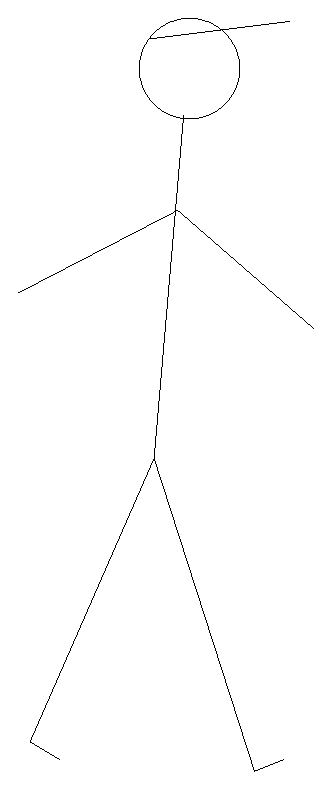
\includegraphics[width=w, height=h]{figura.eps} 
...
\end{document}
\end{verbatim} 

Los par{\'a}metros \verb|width| y \verb|height| son opcionales y puede
omitirse uno para que el sistema escale de acuerdo al par{\'a}metro dado.
Es posible variar la escala completa de la figura o rotarla usando
comandos disponibles en \verb+graphicx+.

\vspace{.3cm}
{\small
\begin{minipage}[t]{5cm}
Una figura aqu\'{\i}:

\begin{center}
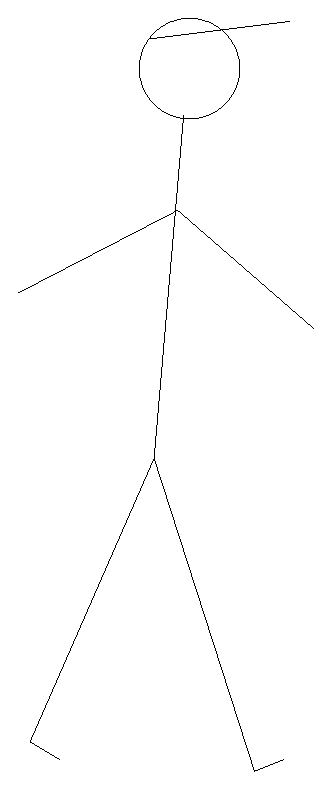
\includegraphics[height=3cm]{figura} % eps to pdf
\end{center}

puede hacer m\'as agradable el texto.
\end{minipage}
\hspace{1.5cm}
\begin{minipage}[t]{5cm}
\begin{verbatim}
Una figura aqu\'{\i}:

\begin{center}
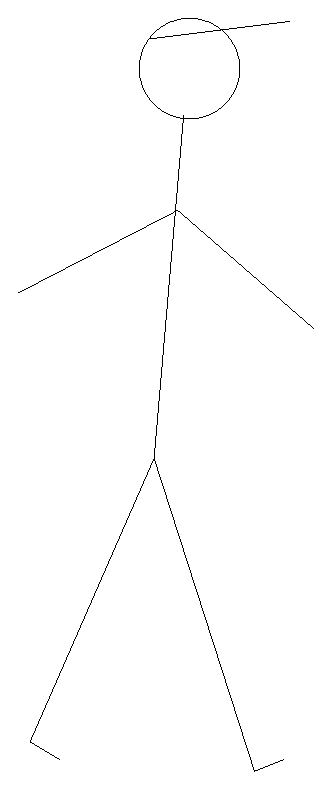
\includegraphics[height=3cm]{figura.eps} 
\end{center}

puede hacer m\'as agradable 
el texto.
\end{verbatim}
\end{minipage}
}
\vspace{.3cm}


En este ejemplo, indicamos s\'olo la altura de la figura
(3cm). El ancho fue determinado de modo que las proporciones de la
figura no fueran alteradas. Si no se especifica ni la altura ni el
ancho, la figura es insertada con su tama\~no natural. 

Observemos tambi\'en que pusimos la figura en un ambiente
\verb+center+. Esto no es necesario, pero normalmente uno desea que
las figuras est\'en centradas en el texto. 

\subsection{Ambiente {\tt figure}.}

Insertar una figura es una cosa. Integrarla dentro del texto es
otra. Para ello est\'a el ambiente \verb+figure+, que permite:
(a) posicionar la figura autom\'aticamente en un lugar predeterminado o
especificado por el usuario; (b) numerar las figuras; y (c) agregar un
breve texto explicativo junto a la figura.

Coloquemos la misma figura de la secci\'on anterior dentro de un
ambiente \verb+figure+. El input:
\begin{verbatim}
\begin{figure}[h]
\begin{center}
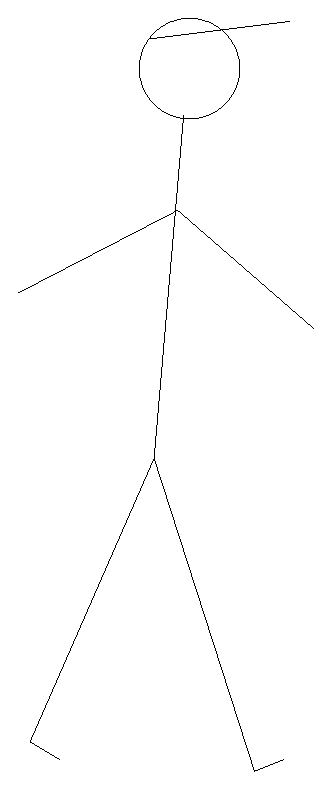
\includegraphics[height=3cm]{figura.eps} 
\end{center}
\caption{Un sujeto caminando.}
\label{caminando}
\end{figure}
\end{verbatim}
da como resultado:
\begin{figure}[h]
\begin{center}
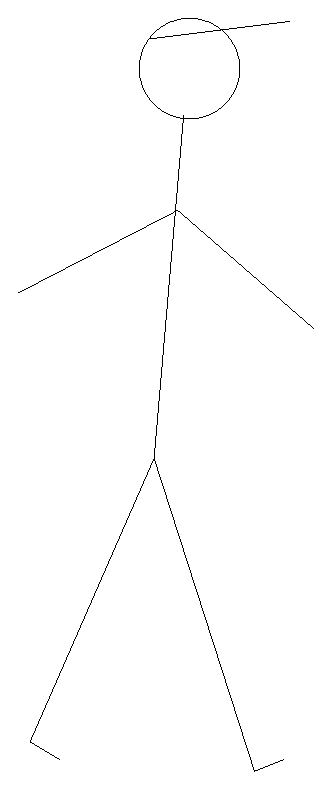
\includegraphics[height=3cm]{figura} % eps to pdf
\end{center}
\caption{Un sujeto caminando.}
\label{caminando}
\end{figure}

\verb+figure+ delimita lo que en \TeX\ se denomina un {\it objeto
  flotante}, es decir, un objeto cuya posici\'on no est\'a determinada
{\it a priori}, y se ajusta para obtener los mejores resultados
posibles. \TeX\ considera (de acuerdo con la tradici\'on), que la
mejor posici\'on para colocar una figura es al principio o al final de
la p\'agina. Adem\'as, lo ideal es que cada p\'agina tenga un cierto
n\'umero m\'aximo de figuras, que  ninguna figura
aparezca en el texto antes de que sea mencionada por primera
vez, y que, por supuesto, las figuras aparezcan en el orden en que son
mencionadas. \'Estas y otras condiciones determinan la posici\'on que un
objeto flotante tenga al final de la compilaci\'on. Uno puede forzar
la decisi\'on de \LaTeX\ con el argumento opcional de \verb+figure+:

\vspace{.3cm}
\begin{tabular}{lll}
\verb+t+&({\em top\/)} & extremo superior de la p\'agina \\
\verb+b+&({\em bottom\/}) & extremo inferior de la p\'agina\\
\verb+h+&({\em here\/}) & aqu\'{\i}, en el punto donde est\'a el
comando\\
\verb+p+&({\em page of floats\/}) & en una p\'agina separada al final
del texto
\end{tabular}
\vspace{.3cm}

El argumento adicional \verb+!+ suprime, para ese objeto flotante
espec\'{\i}fico, cualquier restricci\'on que exista sobre el n\'umero
m\'aximo de objetos flotantes en una p\'agina y el porcentaje de texto
m\'{\i}nimo que debe haber en una p\'agina.

Varios de estos argumentos se pueden colocar simult\'anemente, su
orden dictando la prioridad. Por ejemplo, 
\begin{verbatim}
\begin{figure}[htbp]
...
\end{figure}
\end{verbatim}
indica que la figura se debe colocar como primera prioridad aqu\'{\i}
mismo; si ello no es posible, al comienzo de p\'agina (\'esta o la
siguiente, dependiendo de los detalles de la compilaci\'on), y
as\'{\i} sucesivamente.

Adem\'as, \verb+figure+ numera autom\'aticamente la figura, colocando
el texto ``Figura $N$:'', y \verb+\caption+ permite colocar una
leyenda, centrada en el texto, 
a la figura. Puesto que la numeraci\'on es autom\'atica, las figuras
pueden ser referidas simb\'olicamente con \verb+\label+ y \verb+\ref+
(secci\'on \ref{referencias}). Para que la referencia sea correcta,
\verb+\label+ debe estar dentro del argumento de \verb+\caption+, o
despu\'es, como aparece en el ejemplo de la Figura \ref{caminando}
(\verb+\ref{caminando}+!).

Finalmente, notemos que la figura debi\'o ser centrada
expl\'{\i}citamente con \verb+center+. \verb+figure+ no hace nada
m\'as que tratar la figura como un objeto flotante, proporcionar
numeraci\'on y leyenda. El resto es responsabilidad del autor.   


\section{Cartas.}

Para escribir cartas debemos emplear el estilo \verb+letter+ en vez
del que hemos utilizado hasta ahora, \verb+article+. 
Comandos especiales permiten escribir
una carta, poniendo en lugares adecuados la direcci{\'o}n del remitente,
la fecha, la firma, etc. 

A modo de ejemplo, consideremos el siguiente input:

\begin{verbatim}
\documentclass[12pt]{letter}

\usepackage[spanish]{babel}

\begin{document}

\address{Las Palmeras 3425\\
\~Nu\~noa, Santiago}
\date{9 de Julio de 1998}

\signature{Pedro P\'erez \\ Secretario}

\begin{letter}{Dr.\ Juan P\'erez \\ Las Palmeras 3425 \\ 
\~Nu\~noa, Santiago} 
\opening{Estimado Juan}

A\'un no tenemos novedades.

Parece incre\'{\i}ble, pero los recientes acontecimientos nos han superado,
a pesar de nuestros esfuerzos.  Esperamos que mejores tiempos nos
aguarden.

\closing{Saludos,}
\cc{Arturo Prat \\ Luis Barrios}

\end{letter}
\end{document}
\end{verbatim} 

El resultado se encuentra en la pr\'oxima p\'agina.

\newpage

\ifpdf
   \vspace*{-2.2cm}\hspace*{-2cm}
   \includegraphics[height=28cm]{carta_sola.pdf}
\fi

Observemos que el texto de la carta est{\'a} dentro de un ambiente
\verb+letter+, el cual tiene un argumento obligatorio, donde aparece
el destinatario de la carta (con su direcci{\'o}n 
opcionalmente). 


Los comandos disponibles son:

\vspace{.3cm}
\begin{tabular}{lp{9cm}}
\verb+\address{<direccion>}+ & \verb+<direccion>+ del
remitente. \\[.3cm]
\verb+\signature{<firma>}+ & \verb+<firma>+ del remitente. \\[.3cm]
\verb+\opening{<apertura>}+ & F{\'o}rmula de \verb+<apertura>+.
\\[.3cm] 
\verb+\closing{<despedida>}+ & F{\'o}rmula de \verb+<despedida>+.
\\[.3cm] 
\verb+\cc{<copias>}+ & Receptores de \verb+<copias>+ (si los hubiera).
\end{tabular}
\vspace{.3cm}


Uno puede hacer m{\'a}s de una carta con distintos
ambientes \verb+letter+ en un mismo archivo. Cada una tomar{\'a} el
mismo remitente y firma dados por \verb+\address+ y
\verb+\signature+. Si deseamos que \verb+\address+ o
\verb+\signature+ valgan s{\'o}lo para una carta particular, basta
poner dichos comandos entre el \verb+\begin{letter}+ y el
\verb+\opening+ correspondiente.

Por ejemplo, la siguiente estructura:

\begin{verbatim}
\documentclass[12pt]{letter}
\begin{document}
\address{<direccion remitente>}
\date{<fecha>}
\signature{<firma>}

\begin{letter}{<destinatario 1>}
\opening<apertura 1>
...
\end{letter}

\begin{letter}{<destinatario 2>}
\address{<direccion remitente 2>}
\signature{<firma 2>}
\opening<apertura 2>
...
\end{letter}

\begin{letter}{<destinatario 3>}
\opening<apertura 3>
...
\end{letter}
\end{document}
\end{verbatim}
dar\'a origen a tres cartas con la misma direcci\'on de remitente y
firma, salvo la segunda. 

En todos estos comandos, l{\'\i}neas sucesivas son indicadas con
\verb+\\+. 

%\newpage

%\section{\bibtex}

%\bibtex\ no es una extensi\'on a \LaTeX, sino un programa
%independiente. Por ello, no se utiliza incluyendo en el pre\'ambulo
%una l\'{\i}nea de la forma \verb+\usepackage+, sino que corriendo un
%programa adicional. 

\section{\LaTeX\ y el formato {\tt pdf}.}

Junto con PostScript, otro formato ampliamente difundido
para la transmisi\'on de archivos, especialmente a trav\'es de
Internet, es el formato \verb+pdf+ (Portable Document Format). Para
generar un archivo \verb+pdf+ con \LaTeX\ es necesario compilarlo con
\verb+pdflatex+. As\'{\i}, \verb+pdflatex <archivo>+ generar\'a un
archivo \verb+<archivo>.pdf+ en vez del \verb+<archivo>.dvi+ generado
por el compilador usual. 

Si nuestro documento tiene figuras, s\'olo es posible incluirlas en el
documento si est\'an tambi\'en en formato \verb+pdf+. Por tanto, si
tenemos un documento con figuras en PostScript, debemos introducir dos
modificaciones antes de compilar con \verb+pdflatex+:

\begin{enumerate}[a)]
\item Cambiar el argumento de \verb+\includegraphics+ (secci\'on
  \ref{figuras}) de \verb+<archivo_figura>.eps+\linebreak a
  \verb+<archivo_figura>.pdf+.
\item Convertir las figuras PostScript a \verb+pdf+ (con
  \verb+epstopdf+, por ejemplo). Si tenemos una figura en el archivo
  \verb+<archivo_figura>.eps+, entonces 
\verb+epstopdf <archivo_figura>.eps+ genera el archivo correspondiente
\verb+<archivo_figura>.pdf+.
\end{enumerate}

Observar que el mismo paquete \verb+graphicx+ descrito en la secci\'on
\ref{figuras} para incluir figuras\linebreak \mbox{PostScript} permite, sin
modificaciones, incluir figuras en \verb+pdf+.

\section{Modificando  \LaTeX.}

Esta secci\'on se puede considerar ``avanzada''. Normalmente uno se
puede sentir satisfecho con el desempe\~no de \LaTeX, y no es
necesaria mayor intervenci\'on. A veces, dependiendo de la
aplicaci\'on y del autor, nos gustar\'{\i}a modificar el
comportamiento default. Una alternativa es definir nuevos comandos que
sean \'utiles para nosotros. Si esos nuevos comandos son abundantes, o
queremos reutilizarlos frecuentemente en otros documentos, lo
conveniente es considerar crear un nuevo paquete o incluso una nueva
clase. Examinaremos a continuaci\'on los elementos b\'asicos de estas
modificaciones. 

\subsection{Definici\'on de nuevos comandos.}

\subsubsection{El comando {\tt \bslash newcommand}}

Un nuevo comando se crea con:
\begin{verbatim}
\newcommand{<comando>}{<accion>}
\end{verbatim}

El caso m\'as sencillo es cuando una estructura se repite
frecuentemente en nuestro documento. Por ejemplo, digamos que un
sujeto llamado Crist\'obal no quiere escribir su nombre cada vez que
aparece en su documento:

\vspace{.3cm}
{\small
\begin{minipage}[t]{5cm}
\newcommand{\nombre}{Crist\'obal}
Mi nombre es \nombre. S\'{\i}, como oyes, \nombre. \nombre\ Loyola. 
\end{minipage}
\hspace{1.5cm}
\begin{minipage}[t]{5cm}
\begin{verbatim}
\newcommand{\nombre}{Crist\'obal}
...
\begin{document}
...
Mi nombre es \nombre. S\'{\i}, como oyes, 
\nombre. \nombre\ Loyola. 
\end{verbatim}
\end{minipage}
}
\vspace{.3cm}

Un \verb+\newcommand+ puede aparecer en cualquier parte del
documento, pero lo mejor es que est\'e en el pre\'ambulo, de modo que
sea evidente qu\'e nuevos comandos est\'an disponibles en el presente
documento. Observemos adem\'as que la definici\'on de un comando puede
contener otros comandos (en este caso, \verb+\'+). Finalmente, notamos
que ha sido necesario agregar un espacio expl\'{\i}cito con \verb+\ ,+
al escribir ``Crist\'obal Loyola'': recordemos que un comando comienza
con un backslash y termina con el primer car\'acter que no es
letra. Por tanto, \verb+\nombre Loyola+ ignora el espacio al final de
\verb+\nombre+, y el output ser\'{\i}a ``Crist\'obalLoyola''. 

Tambi\'en es posible definir comandos que funcionen en modo matem\'atico:

\vspace{.3cm}
{\small
\begin{minipage}[t]{5cm}
\newcommand{\vel}{\dot x}

Sea $\vel$ la velocidad, de modo que $\vel(t)> 0$ si $t<0$. 
\end{minipage}
\hspace{1.5cm}
\begin{minipage}[t]{5cm}
\begin{verbatim}
\newcommand{\vel}{\dot x}

Sea $\vel$ la velocidad, de modo que 
$ \vel(t)> 0$ si $t<0$. 
\end{verbatim}
\end{minipage}
}
\vspace{.3cm}

Como \verb+\vel+ contiene un comando matem\'atico (\verb+\dot+),
\verb+\vel+ s\'olo puede aparecer en modo matem\'atico.

Podemos tambi\'en incluir la apertura de modo matem\'atico en la
definici\'on de \verb+\vel+:\linebreak\verb+\newcommand{\vel}{$\dot x$}+. De
este modo, \verb+\vel+ (no \verb+$\vel$+) 
da como output directamente $\dot x$. Sin
embargo, esta soluci\'on no es \'optima, porque la siguiente
ocurrencia de \verb+\vel+ da un error. En efecto, si \verb+\vel+ =
\verb+$\dot x$+, entonces \verb+$ \vel(t)>0$+ = 
\verb+$ $\dot x$> 0$+. 
En tal caso, \LaTeX\ ve que un modo matem\'atico se ha abierto y
cerrado inmediatamente, conteniendo s\'olo un espacio entremedio, y
luego, {\em en modo texto}, viene el comando \verb+\dot+, que es
matem\'atico: \LaTeX\ acusa un error y la compilaci\'on se detiene. 

La soluci\'on a este problema es utilizar el comando
\verb+\ensuremath+, que asegura que haya modo matem\'atico, pero si ya
hay uno abierto, no intenta volverlo a abrir:

\vspace{.3cm}
{\small
\begin{minipage}[t]{5cm}
\newcommand{\vel}{\ensuremath{\dot x}}

Sea \vel\ la velocidad, de modo que $\vel(t)> 0$ si $t<0$. 
\end{minipage}
\hspace{1.5cm}
\begin{minipage}[t]{5cm}
\begin{verbatim}
\newcommand{\vel}{\ensuremath{\dot x}}

Sea \vel\ la velocidad, de modo que 
$ \vel(t)> 0$ si $t<0$. 
\end{verbatim}
\end{minipage}
}
\vspace{.3cm}

Un caso especial de comando matem\'atico es el de operadores tipo
logaritmo (ver Tabla \ref{logaritmo}). Si queremos definir una
traducci\'on al castellano de \verb+\sin+, debemos usar el comando
\verb+\DeclareMathOperator+ disponible via \verb+amsmath+:

\vspace{.3cm}
{\small
\begin{minipage}[t]{5cm}

Ahora podemos escribir en castellano, $\sen x$.
\end{minipage}
\hspace{1.5cm}
\begin{minipage}[t]{5cm}
\begin{verbatim}
\usepackage{amsmath}
\DeclareMathOperator{\sen}{sen}
...
Ahora podemos escribir en castellano, $\sen x$.
\end{verbatim}
\end{minipage}
}
\vspace{.3cm}

A diferencia de \verb+\newcommand+, \verb+\DeclareMathOperator+ s\'olo
puede aparecer en el pre\'ambulo del documento.


Un nuevo comando puede tambi\'en ser usado para ahorrar tiempo de
escritura, reemplazando comandos largos de \LaTeX:


\vspace{.3cm}
{\small
\begin{minipage}[t]{5cm}
\newcommand{\be}{\begin{enumerate}}
\newcommand{\ee}{\end{enumerate}}

\be
\item El primer caso.
\item Ahora el segundo.
\item Y el tercero.
\ee
\end{minipage}
\hspace{1.5cm}
\begin{minipage}[t]{5cm}
\begin{verbatim}
\newcommand{\be}{\begin{enumerate}}
\newcommand{\ee}{\end{enumerate}}

\be
\item El primer caso.
\item Ahora el segundo.
\item Y el tercero.
\ee
\end{verbatim}
\end{minipage}
}
\vspace{.3cm}

\subsubsection{Nuevos comandos con argumentos}

Podemos tambi\'en definir comandos que acepten argumentos. Si el
sujeto anterior, Crist\'obal,  desea escribir cualquier nombre precedido de
``Nombre:'' en it\'alica, entonces puede crear el siguiente comando:

\vspace{.3cm}
{\small
\begin{minipage}[t]{5cm}
\newcommand{\nombre}[1]{\textit{Nombre:} #1}
\nombre{Crist\'obal}

\nombre{Violeta}
\end{minipage}
\hspace{1.5cm}
\begin{minipage}[t]{5cm}
\begin{verbatim}
\newcommand{\nombre}[1]{\textit{Nombre:} #1}

\nombre{Crist\'obal}

\nombre{Violeta}
\end{verbatim}
\end{minipage}
}
\vspace{.3cm}

Observemos que \verb+\newcommand+ tiene un argumento opcional, que
indica el n\'umero de argumentos que el nuevo comando va a
aceptar. Esos argumentos se indican, dentro de la definici\'on del
comando, con \verb+#1+, \verb+#2+, etc. Por ejemplo, consideremos un 
comando que acepta dos argumentos:

\vspace{.3cm}
{\small
\begin{minipage}[t]{5cm}
\newcommand{\fn}[2]{f(#1,#2)}

$$ \fn{x}{y} + \fn{x_3}{y*} = 0 \ . $$
\end{minipage}
\hspace{1.5cm}
\begin{minipage}[t]{5cm}
\begin{verbatim}
\newcommand{\fn}[2]{f(#1,#2)}

$$ \fn{x}{y} + \fn{x_3}{y*} = 0 \ . $$
\end{verbatim}
\end{minipage}
}
\vspace{.3cm}

En los casos anteriores, todos los argumentos son obligatorios. \LaTeX\
permite definir comandos con un (s\'olo un) argumento opcional. Si el
comando acepta $n$ argumentos, el argumento opcional es
el \verb+#1+, y se debe indicar, en un segundo par\'entesis cuadrado,
su valor default. As\'{\i}, podemos modificar el comando \verb+\fn+
del ejemplo anterior para que el primer argumento sea opcional, con
valor default $x$:

\vspace{.3cm}
{\small
\begin{minipage}[t]{5cm}
\newcommand{\fn}[2][x]{f(#1,#2)}

$$ \fn{y} + \fn[x_3]{y*} = 0 \ . $$
\end{minipage}
\hspace{1.5cm}
\begin{minipage}[t]{5cm}
\begin{verbatim}
\newcommand{\fn}[2][x]{f(#1,#2)}

$$ \fn{y} + \fn[x_3]{y*} = 0 \ . $$
\end{verbatim}
\end{minipage}
}
\vspace{.3cm}

\subsubsection{Redefinici\'on de comandos}

Ocasionalmente no nos interesa definir un nuevo comando, sino
redefinir la acci\'on de un comando preexistente. Esto se hace con
\verb+\renewcommand+:

%%%%%%%%%%%%%%%%%%%%%%%%%%%%%%%%%%%%%%%%%%%%%%%%%%%%%%%%%%%%%%%%%%%%%%
%NOTA: El uso de \tt en vez de \verb en este ejemplo es intencional, 
%      porque no se ha discutido este comando
%%%%%%%%%%%%%%%%%%%%%%%%%%%%%%%%%%%%%%%%%%%%%%%%%%%%%%%%%%%%%%%%%%%%%%
\vspace{.3cm}
{\small
\begin{minipage}[t]{5cm}
La antigua versi\'on de {\tt ldots}: \ldots

\renewcommand{\ldots}{\textbullet \textbullet 
\textbullet}

La nueva versi\'on de {\tt ldots}: \ldots
\end{minipage}
\hspace{.5cm}
\begin{minipage}[t]{5cm}
\begin{verbatim}
La antigua versi\'on de  {\tt ldots}: \ldots

\renewcommand{\ldots}{\textbullet \textbullet 
\textbullet}

La nueva versi\'on de {\tt ldots}: \ldots
\end{verbatim}
\end{minipage}
}
\vspace{.3cm}


\subsubsection{P\'arrafos y cambios de l\'{\i}nea dentro de comandos}

En el segundo argumento de \verb+\newcommand+ o \verb+\renewcommand+
puede aparecer cualquier comando de \LaTeX, pero ocasionalmente la
aparici\'on de l\'{\i}neas en blanco (para forzar un cambio de
p\'arrafo) puede provocar problemas. Si ello ocurre, podemos usar
\verb+\par+, que hace exactamente lo mismo. Adem\'as, la definici\'on
del comando queda m\'as compacta:

\vspace{.3cm}
{\small
\begin{minipage}[t]{10cm}
\begin{verbatim}
\newcommand{\comandolargo}{\par Un nuevo comando que incluye un cambio de
  p\'arrafo, porque deseamos incluir bastante texto.\par \'Este es el
  nuevo p\'arrafo.\par}

Observemos en acci\'on el comando: \comandolargo Listo.
\end{verbatim}
\end{minipage}
}
\vspace{.3cm}

\noindent
da como resultado:

%NOTA: El efecto del comando tuvo que ser reproducido manualmente,
% debido a que dentro de minipage \parindent=0, y se ignora el
% \hspace* final por alguna razon
\hspace{3cm}\vspace{.3cm}
{\small
\begin{minipage}[t]{10cm}
\newcommand{\comandolargo}{\newline\hspace*{.5em}
 Un nuevo comando que incluye un cambio de
  p\'arrafo, porque deseamos incluir bastante
  texto.\newline\hspace*{.5em} 
\'Este es el
  nuevo p\'arrafo.\newline}

Observemos en acci\'on el comando: \comandolargo \hspace*{.8em}Listo.
\end{minipage}
}
\vspace{.6cm}

Un ejemplo m\'as \'util ocurre cuando queremos asegurar un cambio de
p\'arrafo, por ejemplo, para colocar un t\'{\i}tulo de secci\'on:

\vspace{.3cm}
{\small
\begin{minipage}[t]{5cm}
\newcommand{\seccion}[1]{\par\vspace{.5cm}{\bf Secci\'on: #1}\par\vspace{.5cm}}

Observemos en acci\'on el comando: \seccion{Ejemplo} Listo.
\end{minipage}
\hspace{1.5cm}
\begin{minipage}[t]{5cm}
\begin{verbatim}
\newcommand{\seccion}[1]{\par\vspace{.5cm}
{\bf Secci\'on: #1}\par\vspace{.5cm}}

Observemos en acci\'on el comando: 
\seccion{Ejemplo} Listo.
\end{verbatim}
\end{minipage}
}
\vspace{.3cm}

Adem\'as de las l\'{\i}neas en blanco, los cambios de l\'{\i}nea
pueden causar problemas dentro de la definici\'on de un nuevo
comando. El ejemplo anterior, con el comando \verb+\seccion+, es un
buen ejemplo: notemos que cuando se defini\'o, pusimos un cambio de
l\'{\i}nea despu\'es de \verb+\vspace{.5cm}+. Ese cambio de
l\'{\i}nea es interpretado (como todos los cambios de l\'{\i}nea) como
un espacio en blanco, y es posible que, bajo ciertas circunstancias,
ese espacio en blanco produzca un output no deseado. Para ello basta
utilizar sabiamente el car\'acter \verb+%+, que permite ignorar todo
el resto de la l\'{\i}nea, {\em incluyendo el cambio de
  l\'{\i}nea}. Ilustremos lo anterior con los siguientes tres
comandos, que subrayan (comando \verb+\underline+) una palabra, y 
difieren s\'olo en el uso de \verb+%+ para borrar
cambios de l\'{\i}nea:

\vspace{.3cm}
{\small
\begin{minipage}[t]{4cm}
\newcommand{\texto}{
Un texto de prueba
}
\newcommand{\textodos}{%
Un texto de prueba
}
\newcommand{\textotres}{%
Un texto de prueba%
}

Notar la diferencia entre: 

\underline{\texto},
\underline{\textodos}, 
y 
\underline{\textotres}.
\end{minipage}
\hspace{1.5cm}
\begin{minipage}[t]{5cm}
\begin{verbatim}
\newcommand{\texto}{
Un texto de prueba
}
\newcommand{\textodos}{%
Un texto de prueba
}
\newcommand{\textotres}{%
Un texto de prueba%
}

Notar la diferencia entre: 

\underline{\texto},
\underline{\textodos}, 
y 
\underline{\textotres}.
\end{verbatim}
\end{minipage}
}
\vspace{.3cm}

\verb+\texto+ conserva espacios en blanco antes y despu\'es del texto,
\verb+\textodos+ s\'olo el espacio en blanco despu\'es del texto, y
\verb+\textotres+ no tiene espacios en blanco alrededor del texto.


\subsubsection{Nuevos ambientes}

Nuevos ambientes en \LaTeX\ se definen con \verb+\newenvironment+:

\begin{verbatim}
\newenvironment{<ambiente>}{<comienzo ambiente>}{<final ambiente>}
\end{verbatim}
define un ambiente \verb+<ambiente>+, tal que \verb+\begin{ambiente}+
  ejecuta los comandos\linebreak \verb+<comienzo ambiente>+, y
  \verb+\end{ambiente}+ ejecuta los comandos \verb+<final ambiente>+. 

Definamos un ambiente que, al comenzar, cambia el font a it\'alica,
pone una l\'{\i}nea horizontal (\verb+\hrule+) y deja un espacio
vertical de .3cm, y que al terminar cambia de p\'arrafo, coloca
\verb+XXX+ en sans serif, deja un nuevo espacio vertical de .3cm, y
vuelve al font roman:


\vspace{.3cm}
{\small
\begin{minipage}[t]{10cm}
\begin{verbatim}
\newenvironment{na}{\it \hrule \vspace{.3cm}}{\par\sf XXX \vspace{.3cm}\rm}
\end{verbatim}
\end{minipage}
}
\vspace{.3cm}

Entonces, con

\vspace{.3cm}
{\small
\begin{minipage}[t]{10cm}
\begin{verbatim}
\begin{na}
  Hola a todos. Es un placer saludarlos en este d\'{\i}a tan especial.

Nunca esper\'e una recepci\'on tan calurosa.
\end{na}
\end{verbatim}
\end{minipage}
}
\vspace{.3cm}

\noindent
obtenemos:

{\small
\begin{center}
\begin{minipage}[t]{10cm}
\newenvironment{na}{\it \hrule \vspace{.3cm}}{\par\sf XXX \vspace{.3cm}\rm}
\begin{na}
  Hola a todos. Es un placer saludarlos en este d\'{\i}a tan especial.

Nunca esper\'e una recepci\'on tan calurosa.
\end{na}
\end{minipage}
\end{center}
}

Los nuevos ambientes tambi\'en pueden ser definidos de modo que
acepten argumentos. Como con \verb+\newcommand+, basta agregar como
argumento opcional a \verb+\newenvironment+ un n\'umero que indique
cu\'antos argumentos se van a aceptar:

\begin{verbatim}
\newenvironment{<ambiente>}[n]{<comienzo ambiente>}{<final ambiente>}
\end{verbatim}
Dentro de \verb+<comienzo ambiente>+, se alude a cada argumento como
\verb+#1+, \verb+#2+, etc. Los argumentos no pueden ser usados en los
comandos de cierre del ambiente (\verb+<final ambiente>+). Por
ejemplo, modifiquemos el ambiente \verb+na+ anterior, de modo que en
vez de colocar una l\'{\i}nea horizontal al comienzo, coloque lo que
le indiquemos en el argumento:

{\small
\begin{verbatim}
\newenvironment{na}[1]{\it #1 \vspace{.3cm}}{\par\sf XXX\hrule\vspace{.3cm}\rm}
\end{verbatim}
}

Ahora us\'emoslo dos veces, cada una con un argumento distinto:

\vspace{.3cm}
{\small
\begin{minipage}[t]{5cm}
\newenvironment{na}[1]{\it #1 \vspace{.3cm}}{\par\sf XXX\hrule\vspace{.3cm}\rm}
El mismo ejemplo anterior, ahora es

\begin{na}{\hrule}
  Hola a todos\ldots%. Es un placer saludarlos en este d\'{\i}a tan especial.
%
%Nunca esper\'e una recepci\'on tan calurosa.
\end{na}

Pero podemos ahora cambiar el comienzo:

\begin{na}{\it XXX}
  Hola a todos\ldots%. Es un placer saludarlos en este d\'{\i}a tan especial.
%
%Nunca esper\'e una recepci\'on tan calurosa.
\end{na}
\end{minipage}
\hspace{1.5cm}
\begin{minipage}[t]{5cm}
\begin{verbatim}
El mismo ejemplo anterior, ahora es

\begin{na}{\hrule}
  Hola a todos...
\end{na}

Pero podemos ahora cambiar el comienzo:

\begin{na}{\it XXX}
  Hola a todos...
\end{na}
\end{verbatim}
\end{minipage}
}
\vspace{.3cm}


\subsection{Creaci\'on de nuevos paquetes y clases}

Si la cantidad de nuevos comandos y/o ambientes que necesitamos en
nuestro documento es suficientemente grande, debemos considerar crear un nuevo
paquete o una nueva clase. Para ello hay que tener clara la diferencia
entre uno y otro. En general, se puede decir que si nuestros comandos
involucran alterar la apariencia general del documento, entonces
corresponde crear una nueva clase (\verb+.cls+). 
Si, por el contrario, deseamos que
nuestros comandos funcionen en un amplio rango de circunstancias, para
diversas apariencias del documento, entonces lo adecuado es un paquete
(\verb+.sty+).

Consideremos por ejemplo la experiencia de los autores de estos
apuntes. Para crear estos apuntes necesitamos b\'asicamente la clase
\verb+book+, con ciertas modificaciones: m\'argenes m\'as peque\~nos,
inclusi\'on autom\'atica de los paquetes \verb+amsmath+, \verb+babel+
y \verb+graphicx+, entre otros, y definici\'on de ciertos ambientes
espec\'{\i}ficos. Todo ello afecta la apariencia
de este documento, cambi\'andola de manera apreciable, pero a la vez
de un modo que en general no deseamos en otro tipo de documento. 
Por ello lo hemos compilado
usando una clase adecuada, llamada \verb+mfm2.cls+. 

Por otro lado, uno de los autores ha necesitado escribir muchas
tareas, pruebas y controles de ayudant\'{\i}a en su vida, y se ha
convencido de que su trabajo es m\'as f\'acil creando una clase
\verb+tarea.cls+, que sirve para esos tres prop\'ositos, definiendo
comandos que le permiten especificar f\'acilmente la fecha de entrega
de la tarea, o el tiempo disponible para una prueba, los nombres del
profesor y el ayudante, etc., una serie de comandos espec\'{\i}ficos
para sus necesidades. 

Sin embargo, tanto en este documento que usa \verb+mfm2.cls+, como
en las tareas y pruebas que usan \verb+tarea.cls+, se utilizan algunos
comandos matem\'aticos que no vienen con \LaTeX, pero que son
recurrentes, como \verb+\sen+ (la funci\'on seno en castellano),
\verb+\modulo+ (el m\'odulo de un vector),
 o \verb+\TLaplace+ (la transformada de Laplace).  Para que estos
 comandos est\'en disponibles en cualquier tipo de documento,
 necesitamos reunirlos en un paquete, en este caso
 \verb+addmath.sty+. De este modo, \verb+mfm2.cls+,
 \verb+tarea.cls+ o cualquier otra clase 
pueden llamar a este paquete y utilizar sus comandos. 

\subsubsection{Estructura b\'asica.}

La estructura b\'asica de un paquete o una clase es: 
\begin{enumerate}[a)]
\item Identificaci\'on: Informaci\'on general (nombre del
  paquete, fecha de creaci\'on, etc.). (Obligatoria.)
\item Declaraciones preliminares: Opcionales, dependiendo del paquete
  o clase en cuesti\'on. 
\item Opciones: Comandos relacionados con el manejo de las opciones
  con las cuales el paquete o clase pueden ser invocados. (Opcional.)
\item M\'as declaraciones: Aqu\'{\i} van los comandos que constituyen
  el cuerpo de la clase o paquete. (Obligatoria: si no hay ninguna
  declaraci\'on, el paquete o clase no hace nada, naturalmente.)
\end{enumerate}

La identificaci\'on est\'a consituida por las siguientes dos
l\'{\i}neas, que deben ir al comienzo del archivo:
\begin{verbatim}
\NeedsTeXFormat{LaTeX2e}
\ProvidesPackage{<paquete>}[<fecha> <otra informacion>]
\end{verbatim}

La primera l\'{\i}nea indica a \LaTeX\ que \'este es un archivo para
\LaTeXe. La segunda l\'{\i}nea especifica que se trata de un paquete,
indicando el nombre del mismo (es decir, el nombre del archivo sin
extensi\'on) y, opcionalmente, la fecha (en formato 
\verb+YYYY/MM/DD+) y otra informaci\'on relevante. Por ejemplo,
nuestro paquete \verb+addmath.sty+ comienza con las l\'{\i}neas:
\begin{verbatim}
\NeedsTeXFormat{LaTeX2e}
\ProvidesPackage{addmath}[1998/09/30 Macros matematicos adicionales (VM)]
\end{verbatim}

Si lo que estamos definiendo es una clase, usamos el comando
\verb+\ProvidesClass+. Para nuestra clase \verb+mfm2.cls+: 
\begin{verbatim}
\NeedsTeXFormat{LaTeX2e}
\ProvidesClass{mfm2}[2002/03/25 Estilo para apuntes MFM II (VM)]
\end{verbatim}

A continuaci\'on de la identificaci\'on vienen los comandos que
se desean incorporar a trav\'es de este paquete o clase. 

Como hemos dicho, \verb+addmath.sty+ contiene muchos nuevos comandos
matem\'aticos que consideramos necesario definir mientras
escrib\'{\i}amos estos apuntes. Veamos los contenidos de una versi\'on
simplificada de dicho paquete:
\begin{verbatim}
\NeedsTeXFormat{LaTeX2e}
\ProvidesPackage{addmath}[1998/09/30 Macros matematicos adicionales (VM)]

\newcommand{\prodInt}[2]{\ensuremath \left(\, #1\, |\, #2\, \right ) }
\newcommand{\promedio}[1]{\langle #1 \rangle}
\newcommand{\intii}{\int_{-\infty}^{\infty}}
\newcommand{\grados}{\ensuremath{^\circ}}
\newcommand{\Hipergeometrica}[4]{{}_2F_1\left (#1, #2, #3\, ; #4\right )}
...
\end{verbatim}

De este modo, incluyendo en nuestro documento el paquete con
\verb+\usepackage{addmath}+, varios nuevos comandos est\'an
disponibles:

$$
\begin{array}{lcl}
 \prodInt{x}{y}&&\mbox{\tt \bslash prodInt\{x\}\{y\}}  \\[.2cm]
 \promedio{x} &&\mbox{\tt \bslash promedio\{x\}}   \\[.2cm]
\displaystyle \intii dz\, f(z)&&\mbox{\tt \bslash intii dz\bslash, f(z)} \\[.2cm]
\angle\, ABC = 90\grados && \mbox{\tt \bslash angle\bslash, 
ABC = 90\bslash grados}\\[.2cm]
\Hipergeometrica{a}{b}{c}{d} &&\mbox{\tt \bslash Hipergeometrica\{a\}\{b\}\{c\}\{d\}} 
\end{array}
$$

\subsubsection{Incluyendo otros paquetes y clases}

Los comandos \verb+\RequirePackage+ y \verb+\LoadClass+ permiten
cargar un paquete o una clase, respectivamente.\footnote{Estos
  comandos s\'olo se pueden usar en un archivo {\tt .sty} o {\tt
    .cls} Para documentos normales, la manera de cargar un paquete es
  {\tt \bslash usepackage}, y para cargar una clase es {\tt \bslash
    documentclass}.}. Esto es de gran utilidad, pues permite construir
un nuevo paquete o clase aprovechando la funcionalidad de otros ya
existentes. 

As\'{\i}, nuestro paquete \verb+addmath.sty+ define bastantes
comandos, pero nos gustar\'{\i}a definir varios m\'as que s\'olo
pueden ser creados con las herramientas de \amslatex/. Cargamos
entonces en \verb+addmath.sty+ el paquete \verb+amsmath+ y otros
relacionados, y estamos en condiciones de crear m\'as comandos:

\begin{verbatim}
\NeedsTeXFormat{LaTeX2e}
\ProvidesPackage{addmath}[1998/09/30 Macros matematicos adicionales (VM)]

\RequirePackage{amsmath}
\RequirePackage{amssymb}
\RequirePackage{euscript}
...
\newcommand{\norma}[1]{\ensuremath \left\lVert\, #1 \,\right\rVert}
\newcommand{\intC}{{\sideset{^*}{}\int}} 
\DeclareMathOperator{\senh}{senh}
...
\end{verbatim}
Por ejemplo:

$$
\begin{array}{lcl}
 \norma{x}&&  \text{\tt \bslash norma\{x\}} \\[.2cm]
\intC dz \, f(z)&&\text{\tt \bslash intC dz \bslash, f(z)}  \\[.2cm]
\senh (2y) && \text{\tt \bslash senh (2y)}   
\end{array}
$$

La posibilidad de basar un archivo \verb+.sty+ o \verb+.cls+ en otro
es
 particularmente importante para una clase, ya que
 contiene una gran cantidad de comandos y definiciones
necesarias para compilar el documento exitosamente. Sin embargo, un
usuario normal, aun cuando desee definir una nueva clase, estar\'a
interesado en modificar s\'olo parte del comportamiento. Con
\verb+\LoadClass+, dicho usuario puede cargar la clase sobre la cual
se desea basar, y luego introducir las modificaciones necesarias,
facilitando enormemente la tarea.

Por ejemplo, al preparar este documento fue claro desde el comienzo
que se necesitaba esencialmente la clase \verb+book+, ya que
ser\'{\i}a un texto muy extenso, pero tambi\'en era claro que se
requer\'{\i}an ciertas modificaciones. Entonces, en nuestra clase
\verb+mfm2.cls+ lo primero que hacemos es cargar la clase \verb+book+,
m\'as algunos paquetes necesarios (incluyendo nuestro \verb+addmath+), 
y luego procedemos a modificar o a\~nadir comandos:

\begin{verbatim}
\NeedsTeXFormat{LaTeX2e}
\ProvidesClass{mfm2}[2002/03/25 Estilo para apuntes MFM II (VM)]

\LoadClass[12pt]{book}

\RequirePackage[spanish]{babel}
\RequirePackage{enumerate}
\RequirePackage{addmath}
\end{verbatim}

En un archivo \verb+.sty+ o un \verb+.cls+ se pueden cargar varios
paquetes con \verb+\RequirePackage+. \verb+\LoadClass+, en cambio,
s\'olo puede aparecer en un \verb+.cls+, y s\'olo es posible usarlo
una vez (ya que normalmente clases distintas son incompatibles entre
s\'{\i}). 

\subsubsection{Manejo de opciones}

En el \'ultimo ejemplo anterior, la clase \verb+mfm2+ carga la clase
\verb+book+ con la opci\'on \verb+12pt+. Esto significa que si nuestro
documento comienza con \verb+\documentclass{mfm2}+, ser\'a compilado
de acuerdo a la clase \verb+book+, en 12 puntos. No es posible cambiar
esto desde nuestro documento. Ser\'{\i}a mejor que pudi\'eramos
especificar el tama\~no de letra fuera de la clase, de modo que
\verb+\documentclass{mfm2}+ d\'e un documento en 10 puntos, y
\verb+\documentclass[12pt]{mfm2}+ uno en 12 puntos. Para lograr esto
hay que poder pasar opciones desde la clase \verb+mfm2+ a
\verb+book+. 

El modo m\'as simple de hacerlo es con
\verb+\LoadClassWithOptions+. Si \verb+mfm2.cls+ ha sido llamada con
opciones \verb+<opcion1>,<opcion2>, etc.+, entonces \verb+book+ ser\'a
llamada con las mismas opciones. Por tanto, basta modificar en
\verb+mfm2.cls+ la l\'{\i}nea \verb+\LoadClass[12pt]{book}+ por:
\begin{verbatim}
\LoadClassWithOptions{book}
\end{verbatim}


\verb+\RequirePackageWithOptions+ es el comando an\'alogo para
paquetes. Si una clase o un paquete llaman a un paquete
\verb+<paquete_base>+  y desean
pasarle todas las opciones con las cuales han sido invocados, basta
indicarlo con:
\begin{verbatim}
\RequirePackageWithOptions{<paquete_base>}
\end{verbatim}

El ejemplo anterior puede ser suficiente en muchas ocasiones, pero en
general uno podr\'{\i}a llamar a nuestra nueva clase, \verb+mfm2+, con
opciones que no tienen nada que ver con \verb+book+. Por ejemplo,
podr\'{\i}amos llamarla con opciones \verb+spanish,12pt+. En tal caso,
deber\'{\i}a pasarle \verb+spanish+ a babel, y \verb+12pt+ a
book. M\'as a\'un, podr\'{\i}amos necesitar definir una {\em nueva\/}
opci\'on, que no existe en ninguna de las clases o paquetes cargados
por \verb+book+, para modificar el comportamiento de \verb+mfm2.cls+
de cierta manera espec\'{\i}fica no prevista. Estas dos tareas,
discriminar entre opciones antes de pasarla a alg\'un paquete
determinado, y crear nuevas opciones, constituyen un manejo m\'as
avanzado de opciones. A continuaci\'on revisaremos un ejemplo
combinado de ambas tareas, extraido de la clase con la cual compilamos
este texto, \verb+mfm2.cls+.

La idea es poder llamar a \verb+mfm2+ con una opci\'on adicional
\verb+keys+, que permita agregar al \verb+dvi+ informaci\'on sobre las
etiquetas (dadas con \verb+\label+) de ecuaciones, figuras, etc., que
aparezcan en el documento (veremos la utilidad y un ejemplo de esto
 m\'as adelante). Lo primero es {\em declarar\/} una nueva opci\'on,
 con:
\begin{verbatim}
\DeclareOption{<opcion>}{<comando>}
\end{verbatim}
\verb+<opcion>+ es el nombre de la nueva opci\'on a declarar, y
\verb+<comando>+ es la serie de comandos que se ejecutan cuando dicha
opci\'on es especificada. 

As\'{\i}, nuestro archivo \verb+mfm2.cls+ debe ser modificado:
\begin{verbatim}
\NeedsTeXFormat{LaTeX2e}
\ProvidesClass{mfm2}[2002/03/25 Estilo para apuntes MFM II (VM)]
...
\DeclareOption{keys}{...}
...
\ProcessOptions\relax
...
\end{verbatim}

Observamos que despu\'es de declarar la o las opciones (en este caso
\verb+keys+), hay que {\em procesarlas}, con
\verb+\ProcessOptions+.\footnote{{\tt \bslash relax} es un comando de
    \TeX\ que, esencialmente, no hace nada, ni siquiera introduce un
    espacio en blanco, y es \'util incluirlo en puntos cr\'{\i}ticos
    de un documento, como en este ejemplo.}} 

Las l\'{\i}neas anteriores permiten que \verb+\documentclass{mfm2}+ y
\verb+\documentclass[keys]{mfm2}+ sean ambas v\'alidas, ejecut\'andose
o no ciertos comandos dependiendo de la forma utilizada. 

Si ahora queremos que \verb+\documentclass[keys,12pt]{mfm2}+ sea una
l\'{\i}nea v\'alida, debemos procesar \verb+keys+ dentro de
\verb+mfm2.cls+, y pasarle a \verb+book.cls+ las opciones
restantes. El siguiente es el c\'odigo definitivo:
\begin{verbatim}
\NeedsTeXFormat{LaTeX2e}
\ProvidesClass{mfm2}[2002/03/25 Estilo para apuntes MFM II (VM)]
\newif\ifkeys\keysfalse
\DeclareOption{keys}{\keystrue}
\DeclareOption*{\PassOptionsToClass{\CurrentOption}{book}}
\ProcessOptions\relax
\LoadClass{book}

\RequirePackage[spanish]{babel}
\RequirePackage{amsmath}
\RequirePackage{theorem}
\RequirePackage{epsfig}
\RequirePackage{ifthen}
\RequirePackage{enumerate}
\RequirePackage{addmath}
\ifkeys\RequirePackage[notref,notcite]{showkeys}\fi

<nuevos comandos de la clase mfm2.cls>
\end{verbatim}

Sin entrar en demasiados detalles, digamos que la opci\'on \verb+keys+
tiene el efecto de hacer que una cierta variable l\'ogica
\verb+\ifkeys+, sea verdadera (cuarta l\'{\i}nea del c\'odigo). La
siguiente l\'{\i}nea (\verb+\DeclareOption*...+) hace que todas las
opciones que no han sido procesadas (\verb+12pt+, por ejemplo)
se pasen a la clase \verb+book+. A continuaci\'on se procesan las
opciones con \verb+\ProcessOptions+, y finalmente se carga la clase
\verb+book+. 

Las l\'{\i}neas siguientes cargan todos los paquetes necesarios, y
finalmente se encuentran todos los nuevos comandos y definiciones
que queremos incluir en \verb+mfm2.cls+. 

Observemos que la forma particular en que se carga el paquete
\verb+showkeys+. \'Esa es precisamente la funci\'on de la opci\'on
\verb+keys+ que definimos: \verb+showkeys.sty+ se carga con ciertas
opciones s\'olo si se da la opci\'on \verb+keys+. 

?`Cu\'al es su
efecto? Consideremos el siguiente texto de ejemplo, en que \verb+mfm2+
ha sido llamada sin la opci\'on \verb+keys+:
\begin{verbatim}
\documentclass[12pt]{mfm2}              
\begin{document}
La opci\'on \verb+keys+ resulta muy \'util cuando tengo objetos numerados
autom\'aticamente, como una ecuaci\'on:
\begin{equation}
  \label{newton}
  \vec F = m \vec a \ . 
\end{equation}
y luego quiero referirme a ella: Ec.\  \eqref{newton}.
\end{verbatim}

En el primer caso, se ha compilado sin la opci\'on \verb+keys+, y en
el segundo con ella. El efecto es que, si se usa un \verb+\label+ en
cualquier parte del documento, aparece en el margen derecho una caja
con el nombre de dicha etiqueta (en este caso, \verb+newton+). 
Esto es \'util para cualquier tipo de
documentos, pero lo es especialmente en textos como
 estos apuntes, muy extensos y con
abundantes referencias. En tal caso, tener un modo visual, r\'apido,
de saber los nombres de las ecuaciones sin tener que revisar
trabajosamente el archivo fuente es una gran ayuda. As\'{\i},
versiones preliminares pueden ser compiladas con la opci\'on
\verb+keys+, y la versi\'on final sin ella, para no confesar al lector
nuestra mala memoria o nuestra comodidad.


\newpage


\ifpdf
 \vspace*{-2.2cm}\hspace*{-4cm}
 \includegraphics[height=28cm]{keys_example.pdf}
\fi

\section{Errores y advertencias.}

\subsection{Errores.}

Un mensaje de error t{\'\i}pico tiene la forma:\label{itemie}
\begin{verbatim}
LaTeX error. See LaTeX manual for explanation.
             Type H <return> for immediate help.
! Environment itemie undefined.
\@latexerr ...or immediate help.}\errmessage {#1}
                                                 \endgroup
l.140 \begin{itemie}

?  
\end{verbatim}


La primera l{\'\i}nea nos comunica que \LaTeX\ ha encontrado un
error. A veces los errores tienen que ver con  procesos m{\'a}s
internos, y son encontrados por \TeX. Esta l{\'\i}nea nos informa
qui{\'e}n encontr{\'o} el error. 

La tercera l{\'\i}nea comienza con un signo de exclamaci{\'o}n. {\'E}ste
es el indicador del error. Nos dice de qu{\'e} error se trata.

Las dos l{\'\i}neas siguientes describen el error en t{\'e}rminos de
comandos de bajo nivel.

La l{\'\i}nea 6 nos dice d{\'o}nde ocurri{\'o} el error: la l{\'\i}nea
140 en este caso. Adem{\'a}s nos informa del texto conflictivo:
\verb+\begin{itemie}+.
  
  En realidad, el mensaje nos indica d{\'o}nde \LaTeX\ advirti{\'o} el error
  por primera vez, que no es necesariamente el punto donde el error se
  cometi{\'o}. Pero la gran mayor{\'\i}a de las veces la indicaci{\'o}n es
  precisa. De hecho, es f{\'a}cil darse cuenta, con la tercera l{\'\i}nea\\
  (\verb+Environment itemie undefined+)\\ y la sexta
  (\verb+\begin{itemie}+) que el error consisti{\'o} en escribir
    \verb+itemie+ en vez de \verb+itemize+. La informaci{\'o}n de \LaTeX\ 
    es clara en este caso y nos dice correctamente qu{\'e} ocurri{\'o} y
    d{\'o}nde.

Luego viene un \verb+?+. \LaTeX\ est{\'a} esperando una respuesta de
nosotros. Tenemos varias alternativas. Comentaremos s{\'o}lo cuatro,
t{\'\i}picamente usadas:

\begin{list}{(\alph{enumi})}{\usecounter{enumi}%
\renewcommand{\theenumi}{(\alph{enumi})}}
\item \verb+h <Enter>+

Solicitamos ayuda. \TeX\ nos explica brevemente en qu{\'e} cree {\'e}l
que consiste el error y/o nos da alguna recomendaci{\'o}n.

\item \verb+x <Enter>+

Abortamos la compilaci{\'o}n. Deberemos volver al editor y corregir el
texto. Es la opci{\'o}n m{\'a}s t\'{\i}pica cuando uno tiene ya cierta
experiencia, pues el mensaje basta para reconocer el error.

\item \verb+<Enter>+
\label{Enter}

Ignoramos el error y continuamos la compilaci{\'o}n. \TeX\ hace lo que
puede. En algunos casos esto no tiene consecuencias
graves y podremos llegar hasta el final del archivo sin mayores
problemas. En otros casos, ignorar el error puede provocar que
ulteriores comandos ---perfectamente v{\'a}lidos en principio--- no
sean reconocidos y, as\'{\i}, acumular muchos errores m{\'a}s. Podemos
continuar con \verb+<Enter>+ sucesivos hasta llegar al final de la
compilaci{\'o}n. 

\item \verb+q <Enter>+
\label{q}

La acci{\'o}n descrita en el punto anterior puede llegar a ser tediosa o
infinita. \verb+q+ hace ingresar a \TeX\ en \verb+batchmode+, modo en
el cual la compilaci{\'o}n prosigue ignorando todos los errores hasta
el final del archivo, sin enviar mensajes a pantalla y por ende sin
que debamos darle infinitos \verb+<Enter>+. 

\end{list}

Las opciones \ref{Enter} y \ref{q} son
{\'u}tiles cuando no entendemos los mensajes de error. Como \TeX\ seguir{\'a}
compilando haciendo lo mejor posible, al mirar el \verb+dvi+ puede
que veamos m{\'a}s claramente d{\'o}nde comenzaron a ir mal las cosas y,
por tanto, por qu{\'e}.

\vspace{.3cm}
Como dijimos, \LaTeX\ indica exactamente d{\'o}nde encontr{\'o} el error,
de modo que hemos de ponerle atenci{\'o}n. Por ejemplo, si 
tenemos en nuestro documento la l\'{\i}nea:
\begin{verbatim}
... un error inesperado\fotnote{En cualquier punto.} 
puede decidir...
\end{verbatim}
generar\'{\i}a el mensaje de error:
\begin{verbatim}
! Undefined control sequence.

l.249 ...un error inesperado\fotnote
                                    {En cualquier punto.}
?
\end{verbatim}

En la l\'{\i}nea de localizaci{\'o}n, \LaTeX\ ha cortado el texto
justo despu{\'e}s del comando inexistente. \LaTeX\ no s{\'o}lo indica la
l\'{\i}nea en la cual detect{\'o} el error, sino el punto de ella donde
ello ocurri{\'o}. (En realidad, hizo lo mismo ---cortar la l\'{\i}nea
para hacer resaltar el problema--- en el caso expuesto en la
p{\'a}g.\ \pageref{itemie},  pero ello ocurri{\'o} en medio de comandos
de bajo nivel, as\'{\i} que no era muy informativo de todos modos.)

\subsubsection{Errores m{\'a}s comunes.}
\label{comunes}

Los errores m{\'a}s comunes son:
\begin{list}{\alph{enumi})}{\usecounter{enumi}%
\renewcommand{\theenumi}{\alph{enumi})}}
\item Comando mal escrito.
\label{mal}
\item Par{\'e}ntesis cursivos no apareados.
\label{cursivos}
\item Uso de uno de los caracteres especiales \verb+#+, \verb+$+,
\verb+%+, \verb+&+, \verb+_+, \verb+{+, \verb+}+, \verb+~+, \verb+^+,
\verb+\+ como texto ordinario.
\label{especiales}
\item Modo matem{\'a}tico abierto de una manera y cerrado de otra, o no
cerrado. 
\label{endmath}
\item Ambiente abierto con \verb+\begin...+ y cerrado con un
\verb+\end...+ distinto.
\label{endgroup}
\item Uso de un comando matem{\'a}tico fuera de modo matem{\'a}tico.
\label{mathmode}
\item Ausencia de argumento en un comando que lo espera.
\label{argumento}
\item L\'{\i}nea en blanco en ambiente matem{\'a}tico.
\label{blank}
\end{list}

\subsubsection{Algunos mensajes de error.}

A continuaci{\'o}n, una peque{\~n}a lista de errores (de \LaTeX\ y \TeX)
en orden alfab{\'e}tico, y sus posibles causas.

\begin{list}{}{\setlength{\leftmargin}{0pt}}
\item \verb+*+

Falta \verb+\end{document}+. (Dar \verb+Ctrl-C+ o escribir
\verb+\end{document}+ para salir de la compilaci{\'o}n.)

\item \verb+! \begin{...} ended by \end{...}+

Error \ref{endgroup} de la Sec.\ \ref{comunes}. El nombre del
ambiente en \verb+\end{...}+ puede estar mal escrito, sobra un
\verb+\begin+ o falta un \verb+\end+. 

\item \verb+! Double superscript+ (o \verb+subscript+).

Una expresi{\'o}n como \verb+x^2^3+ o \verb+x_2_3+. Si se desea obtener
${x^2}^3$ (${x_2}_3$), escribir \verb+{x^2}^3+ (\verb+{x_2}_3+). 

\item \verb+! Environment ... undefined.+

\verb+\begin{...}+ con un argumento que corresponde a un ambiente no
definido. 

\item \verb+! Extra alignment tab has been changed.+

En un \verb+tabular+ o \verb+array+ sobra un \verb+&+, falta un
\verb+\\+, o falta una \verb+c+, \verb+l+ {\'o} \verb+r+ en el
argumento obligatorio.

\item \verb+! Misplaced alignment tab character &.+

Un \verb+&+ aparece fuera de un \verb+tabular+ o \verb+array+.

\item \verb+! Missing $ inserted.+

Errores \ref{especiales}, \ref{endmath}, \ref{mathmode}, \ref{blank}
de la Sec.\ \ref{comunes}.

\item \verb+! Missing {+ (o \verb+}+) \verb+inserted.+

Par{\'e}ntesis cursivos no apareados.

\item \verb+! Missing \begin{document}.+

Falta \verb+\begin{document}+ o hay algo incorrecto en el
pre{\'a}mbulo. 

\item \verb+! Missing number, treated as zero.+

Falta un n{\'u}mero donde \LaTeX\ lo espera: \verb+\hspace{}+,
\verb+\vspace cm+,\linebreak \verb+\setlength{\textwidth}{a}+, etc.

\item \verb+! Something's wrong -- perhaps a missing \item.+

Posiblemente la primera palabra despu{\'e}s de un
\verb+\begin{enumerate}+ o\linebreak \verb+\begin{itemize}+ no es \verb+\item+. 

\item \verb+! Undefined control sequence.+

Aparece una secuencia \verb+\<palabra>+, donde \verb+<palabra>+ no es
un comando.

\end{list}

\subsection{Advertencias.}
\label{advertencias}

La estructura de una advertencia de \LaTeX\ es:
\begin{verbatim}
LaTeX warning. <mensaje>.
\end{verbatim}

Algunos ejemplos:

\begin{list}{}{\setlength{\leftmargin}{0pt}}
\item \verb+Label `...' multiply defined.+

Dos \verb+\label+ tienen el mismo argumento.

\item \verb+Label(s) may have changed. Rerun to get cross-references right.+ 

Los n{\'u}meros impresos por \verb+\ref+ y \verb+\pageref+ pueden ser
incorrectos, pues los valores correspondientes cambiaron respecto al
contenido del \verb+aux+ generado en la compilaci{\'o}n anterior.

\item \verb+Reference `...' on page ... undefined.+

El argumento de un \verb+\ref+ o un \verb+\pageref+ no fue definido
por un \verb+\label+.

\end{list}

\TeX\ tambi{\'e}n env\'{\i}a advertencias. Se reconocen porque no
comienzan con \verb+TeX warning+. 

Algunos ejemplos.

\begin{list}{}{\setlength{\leftmargin}{0pt}}
\item \verb+Overfull \hbox ...+

\TeX\ no encontr{\'o} un buen lugar para cortar una l\'{\i}nea, y puso
m{\'a}s texto en ella que lo conveniente.

\item \verb+Overfull \vbox ...+

\TeX\ no encontr{\'o} un buen lugar para cortar una p{\'a}gina, y puso
m{\'a}s texto en ella que lo conveniente.

\item \verb+Underfull \hbox ...+

\TeX\ construy{\'o} una l\'{\i}nea con muy poco material, de modo que
el espacio entre palabras puede ser excesivo.

\item \verb+Underfull \vbox ...+

\TeX\ construy{\'o} una p{\'a}gina con muy poco material, de modo que los
espacios verticales (entre p{\'a}rrafos) pueden ser excesivos.
\end{list}


Las advertencias de \LaTeX\ siempre deben ser atendidas. Una
referencia doblemente definida, o no compilar por segunda vez cuando
\LaTeX\ lo sugiere, generar{\'a} un resultado incorrecto en el
\verb+dvi+. Una referencia no definida, por su parte, hace aparecer
un signo {\bf ??} en el texto final. Todos resultados no deseados, por
cierto. 

Las advertencias de \TeX\ son menos decisivas. Un overfull o
underfull puede redundar en que alguna palabra se salga del margen
derecho del texto, que el espaciado entre palabras en una l\'{\i}nea
sea excesivo, o que el espacio vertical entre p{\'a}rrafos sea
demasiado. Los est{\'a}ndares de calidad de \TeX\ son altos, y por eso
env\'{\i}a advertencias frecuentemente. Pero generalmente los
defectos en el resultado final son imperceptibles a simple vista, o
por lo menos no son suficientes para molestarnos realmente. A veces
s\'{\i}, por supuesto, y hay que estar atentos. Siempre conviene
revisar el texto y prestar atenci{\'o}n a estos detalles, aunque ello
s{\'o}lo tiene sentido al preparar la versi{\'o}n definitiva del
documento. 




% Local Variables: 
% TeX-master: "mfm"
% End: 
